\documentclass[12pt,a4paper]{article}
\usepackage{fontspec,polyglossia}
\setdefaultlanguage{russian}
\setmainfont{Times New Roman}
\newfontfamily\cyrillicfont{Times New Roman}
\setmonofont{Courier New}
\newfontfamily\cyrillicfonttt{Courier New}
\usepackage{amsmath,amssymb,mathtools,graphicx,array,longtable,tabularx,float,caption,geometry,titlesec,indentfirst,enumitem,listings,tikz,multicol,needspace}
\usetikzlibrary{arrows.meta,positioning,calc}
\usepackage[hidelinks]{hyperref}
\geometry{left=25mm,right=15mm,top=20mm,bottom=20mm}
\setlength{\parindent}{1.25cm}\setlength{\parskip}{3pt}\linespread{1.08}
\setlength{\emergencystretch}{3em}
\titleformat{\section}{\bfseries\normalsize}{\thesection.}{0.5em}{}
\titleformat{\subsection}{\bfseries\normalsize}{\thesubsection.}{0.5em}{}
\titlespacing*{\section}{0pt}{10pt}{5pt}\titlespacing*{\subsection}{0pt}{7pt}{4pt}
\captionsetup{labelsep=endash,font=small,justification=centering}
\addto\captionsrussian{\renewcommand{\figurename}{График}}
\setlist{nosep,leftmargin=1.2cm}
\lstset{basicstyle=\ttfamily\fontsize{9}{10.5}\selectfont,breaklines=true,columns=fullflexible,keepspaces=true,showstringspaces=false,frame=none}
\newcommand{\concl}[1]{\par\noindent\textit{Вывод.} #1\par}
\hypersetup{pdftitle={УИР 3. Исследование СМО и СеМО},pdfauthor={Якименко Владислав Игоревич}}
\begin{document}
\begin{titlepage}\centering
Федеральное государственное автономное образовательное учреждение\\
высшего образования\\
«Национальный исследовательский университет ИТМО»\\[5mm]
Факультет программной инженерии и компьютерной техники
\vfill
{\large\bfseries Учебно-исследовательская работа № 3}\\[5mm]
{\large\bfseries «Исследование СМО и СеМО»}\\[5mm]
по дисциплине «Моделирование»\\[3mm]
Выборка УИР 1 -- 16; СМО из УИР 2 -- СИСТЕМА\_2; СеМО -- 6/6
\vfill
\begin{flushright}\begin{tabular}{ll}
Выполнил: & Якименко Владислав Игоревич\\
Группа: & P3313\\
Проверил: & Авксентьева Елена Юрьевна
\end{tabular}\end{flushright}
\vfill Санкт-Петербург\\2026
\end{titlepage}
\setcounter{page}{2}
\begin{center}\textbf{Часть 1 «Исследование свойств систем массового обслуживания (СМО)»}\end{center}
\section{Постановка задачи и исходные данные}
\noindent\textbf{Цель работы.} Исследование свойств систем и сетей массового обслуживания с однородным потоком заявок в среде имитационного моделирования GPSS при различных предположениях о параметрах структурно-функциональной организации и нагрузки в соответствии с формируемой исследователем (студентом) программой исследований.

Постановка задачи и обозначения взяты из задания «Исследование СМО и СеМО», редакция от 19.10.25, и приложенного теоретического материала. Работа содержит две части: исследование свойств СМО и исследование свойств СеМО.

В первой части используется СИСТЕМА\_2, выбранная в УИР 2 по максимальной производительности, и числовая последовательность варианта 16 из УИР 1. Во второй части \(A=6\) и \(B=6\) получены по последней цифре номера 16 в списке группы. В таблице 2 задания имеются строки 1--10; использование строки 6 подтверждено при выдаче варианта.

\noindent\textbf{Среда моделирования.} Исследования выполнены в GPSS World Core. Модели прошли трансляцию; стандартные отчёты сохранены. Таблицы и графики построены по результатам GPSS. Python используется для обработки этих отчётов и независимого контрольного расчёта. Исходные проекты, результаты отдельных повторений и стандартные отчёты приложены к работе.

\subsection{СМО из УИР 2}
Имеются три прибора с отдельными накопителями. Заявка направляется к одному прибору и теряется при его заполнении. Повторного выбора прибора нет. Дисциплина обслуживания FIFO.

Сохраняются обозначения задания: \(K\) -- количество обслуживающих приборов; \(E\) -- ёмкость накопителя; \(a\) -- средний интервал между поступающими в систему заявками; \(b\) -- средняя длительность обслуживания; КВ -- коэффициент вариации длительности обслуживания. В формулах, как в теоретическом материале, коэффициент вариации обозначается \(\nu\), его разновидности -- \(\nu_a,\nu_b,\nu_w,\nu_u\). Индекс \(j\) обозначает отдельный прибор или узел. Вектор \((E_1,E_2,E_3)=(2,1,0)\) задаёт три отдельных накопителя; их нельзя заменять одним общим накопителем ёмкости 3.

\begin{center}\small\renewcommand{\arraystretch}{1.3}
\begin{tabular}{|l|c|c|c|}\hline
Параметр & П1 & П2 & П3\\\hline
Число приборов \(K_j\) & 1 & 1 & 1\\\hline
Ёмкость накопителя \(E_j\) & 2 & 1 & 0\\\hline
Вероятность направления \(\alpha_j\) & 0,30 & 0,45 & 0,25\\\hline
Закон обслуживания & \(M\) & \(M\) & \(E_2\)\\\hline
Среднее обслуживание \(b\), с & 5 & 5 & 5\\\hline
\end{tabular}\end{center}


Контрольное сравнение с УИР 2 выполняется при \(\lambda=0{,}8\;\text{с}^{-1}\), \(a=1/\lambda=1{,}25\;\text{с}\). Далее средний входной интервал заменяется средним исходной выборки УИР 1.
\begin{equation}
a=\frac1{300}\sum_{i=1}^{300}X_i=8{,}020778\;\text{с},\qquad
\widetilde\sigma=22{,}592719\;\text{с},\qquad
\widetilde\nu=\frac{\widetilde\sigma}{a}=2{,}816774.
\end{equation}
Исходная выборка взята из листа «1-50», столбца с заголовком 16, строки 2--301. Все 300 исходных значений сохранены в \texttt{data/trace16.csv}.
\section{Модель, измерения и план экспериментов}
\subsection{Событийная модель}
Календарь событий ведёт GPSS. Входной транзакт-генератор задерживается на интервал между поступлениями (\texttt{ADVANCE}); \texttt{SPLIT} создаёт заявку, \texttt{TRANSFER} выбирает направление. Условие приёма проверяется блоком \texttt{TEST}:
\begin{equation}
C_j(t_i)+Q_j(t_i)<K_j+E_j.
\end{equation}
Здесь \(C_j\) -- число занятых приборов направления, \(Q_j\) -- длина его очереди. При отказе увеличивается счётчик \texttt{LOST}; заявка удаляется блоком \texttt{TERMINATE 1}. Принятая заявка проходит \texttt{QUEUE}, \texttt{ENTER}, \texttt{DEPART}, \texttt{ADVANCE}, \texttt{LEAVE}. Её начало и окончание обслуживания обозначены \(s_i,d_i\):
\begin{gather}
s_i=\max(t_i,f_{j,\min}),\qquad d_i=s_i+B_i,\\
W_i=s_i-t_i,\qquad U_i=d_i-t_i,\qquad U_i=W_i+B_i.
\end{gather}
Здесь \(t_i\) -- момент поступления, \(f_{j,\min}\) -- ближайшее освобождение прибора выбранного узла, \(B_i\) -- сгенерированная длительность обслуживания. При нескольких приборах используется первый освобождающийся прибор.

Для окна наблюдения длительности \(T\) GPSS интегрирует занятость и длину очереди. Пусть \(N_{\text{обс}}\) -- число завершённых обслуживаний, \(N_{\text{пот}}\) -- число отказов, \(N=N_{\text{обс}}+N_{\text{пот}}\) -- число прошедших заявок. Тогда
\begin{gather}
\widehat\pi=\frac{N_{\text{пот}}}{N},\qquad
\widehat\lambda'=\frac{N_{\text{обс}}}{T},\qquad
\widetilde w=\frac1{n_w}\sum_{i=1}^{n_w} W_i,\qquad
\widetilde u=\frac1{n_u}\sum_{i=1}^{n_u} U_i,\\
\widetilde l_j=\frac1T\int_0^TQ_j(t)\,dt,\qquad
\widetilde\rho_j=\frac1{K_jT}\int_0^TC_j(t)\,dt.
\end{gather}
Ожидание регистрируется при начале обслуживания (таблица \texttt{TW}), пребывание -- при завершении (\texttt{TU}). Их количества \(n_w,n_u\) берутся из частот таблиц. Незавершённые к моменту остановки заявки остаются в модели. Поэтому числа поступивших, начавших и завершивших обслуживание заявок на конечном горизонте могут различаться. Погрешность границ учитывается при проверке равенств Литтла.

\subsection{Точность и воспроизводимость}
В основных сериях выполняются восемь независимых повторений. Доверительный интервал 0,95 оценивается по средним повторений, что учитывает зависимость последовательных времён ожидания внутри одного прогона.
\begin{equation}
\overline z=\frac1R\sum_{r=1}^Rz_r,\quad
s_z^2=\frac1{R-1}\sum_{r=1}^R(z_r-\overline z)^2,\quad
\overline z\pm\varepsilon_z,\qquad
\varepsilon_z=t_{0{,}975;R-1}\frac{s_z}{\sqrt R}+\Delta_{\text{окр}}.
\end{equation}
Для СМО в каждом повторении пропускаются 10\,000 прошедших заявок разгона и измеряются следующие 60\,000; при контрольном сравнении -- 12 повторений по 200\,000. Для ЗСеМО используются 10\,000 циклов разгона и 30\,000 измеряемых циклов, для РСеМО -- 20\,000 и 40\,000 соответственно. Перед независимым повторением выполняются \texttt{CLEAR} и \texttt{RMULT}; перед измерением после разгона -- \texttt{RESET}, сохраняющий текущее состояние. Начальные числа генераторов фиксированы: \(601+1000r+i\) для СМО и \(661+1000r+i\) для сети, \(r=0,\ldots,R-1\), \(i=0,\ldots,6\).

Большинство средних GPSS печатает с шагом 0,001. К статистическому полуинтервалу добавлен предельный допуск округления: 0,0005 для отдельного среднего, 0,0015 для суммы трёх длин очередей. Производительность и вероятность потери вычисляются из целых счётчиков и модельного времени.

Команда \texttt{START N} задаёт число прохождений \texttt{TERMINATE 1}: завершений обслуживания и отказов. При исследовании переходного процесса выполняется последовательность \texttt{START} с приращениями счётчика, а отчёты сохраняются при накопленных \(N=10,20,\ldots,100000\). Для нового независимого повторения модель полностью очищается. Вспомогательный алгоритм Python проверяется отдельно и не заменяет результаты GPSS.

\subsection{Предлагаемая нагрузка и фактическая загрузка}
При сохранении маршрутизации загрузка отдельных приборов различается. Для согласованного изменения обслуживания введена максимальная предлагаемая нагрузка
\begin{equation}
y_j=\frac{\alpha_j b}{aK_j},\qquad y_{\max}=\max_jy_j,
\qquad b=\frac{y_{\max}a}{0{,}45}\quad(K_j=1).
\end{equation}
Исследуются \(y_{\max}=0{,}5;\,0{,}75;\,0{,}95;\,0{,}99\). Из-за отказов фактическая загрузка \(\rho_j\) меньше предлагаемой. Например, для простейшего потока при \(y_{\max}=0{,}99\) средняя по трём приборам загрузка составляет около 0,53. Эти величины различаются во всех таблицах. Дополнительная серия ниже обеспечивает значения именно фактической средней загрузки 0,5; 0,75; 0,95 и 0,99 для простейшего потока.


\noindent\begin{minipage}{\textwidth}\noindent\hfill Форма 1\par\begin{center}\textbf{Описание исследуемых вариантов организации системы}\end{center}
\begin{center}\small\renewcommand{\arraystretch}{1.3}
\resizebox{\textwidth}{!}{\begin{tabular}{|l|c|c|c|c|c|c|}\hline
Номер варианта & 1 & 2 & 3 & 4 & 5 & 6\\\hline
Количество приборов & 3 & 3 & 3 & 3 & 3 & 3\\\hline
Ёмкость накопителя & \((2,1,0)\) & \((2,1,0)\) & \((2,1,0)\) & \((2,1,0)\) & \((2,1,0)\) & \((2,1,0)\)\\\hline
\shortstack{Интервалы между заявками\\входящего потока: ср. значение} & 8,0208 & 8,0208 & 8,0208 & 8,0208 & 8,0208 & 8,0208\\\hline
Вид потока & Т & А & П & Т & А & П\\\hline
\shortstack{Длительность обслуживания\\заявок: ср. значение} & 8,9120 & 8,9120 & 8,9120 & 13,3680 & 13,3680 & 13,3680\\\hline
Коэф-т вариации & \((1;1;\frac1{\sqrt2})\) & \((1;1;\frac1{\sqrt2})\) & \((1;1;\frac1{\sqrt2})\) & \((1;1;\frac1{\sqrt2})\) & \((1;1;\frac1{\sqrt2})\) & \((1;1;\frac1{\sqrt2})\)\\\hline
\end{tabular}}\end{center}

\end{minipage}\par\medskip
\noindent\begin{minipage}{\textwidth}\noindent\hfill Форма 1\par\begin{center}\textbf{Описание исследуемых вариантов организации системы}\end{center}
\begin{center}\small\renewcommand{\arraystretch}{1.3}
\resizebox{\textwidth}{!}{\begin{tabular}{|l|c|c|c|c|c|c|}\hline
Номер варианта & 7 & 8 & 9 & 10 & 11 & 12\\\hline
Количество приборов & 3 & 3 & 3 & 3 & 3 & 3\\\hline
Ёмкость накопителя & \((2,1,0)\) & \((2,1,0)\) & \((2,1,0)\) & \((2,1,0)\) & \((2,1,0)\) & \((2,1,0)\)\\\hline
\shortstack{Интервалы между заявками\\входящего потока: ср. значение} & 8,0208 & 8,0208 & 8,0208 & 8,0208 & 8,0208 & 8,0208\\\hline
Вид потока & Т & А & П & Т & А & П\\\hline
\shortstack{Длительность обслуживания\\заявок: ср. значение} & 16,9328 & 16,9328 & 16,9328 & 17,6457 & 17,6457 & 17,6457\\\hline
Коэф-т вариации & \((1;1;\frac1{\sqrt2})\) & \((1;1;\frac1{\sqrt2})\) & \((1;1;\frac1{\sqrt2})\) & \((1;1;\frac1{\sqrt2})\) & \((1;1;\frac1{\sqrt2})\) & \((1;1;\frac1{\sqrt2})\)\\\hline
\end{tabular}}\end{center}

\end{minipage}\par\medskip

Числа \(a,b\) в форме 1 указаны в секундах. Для трёх отдельных направлений ёмкость накопителя и КВ обслуживания записаны вектором. Варианты 1--12 относятся к обязательному сравнению потоков Т, А и П. Остальные серии изменяют один фактор: закон обслуживания \(M,E_2,H_2\); общую для каждого накопителя ёмкость \(E=0,1,2,4,8,16,32,64,128,256\); число приборов \(K_j=1,2,3\) в каждом направлении. Точные параметры каждого опыта сохранены в таблицах CSV и текстах GPSS.


\section{Сравнение с марковской моделью УИР 2}
Структура и параметры контрольного эксперимента полностью совпадают с СИСТЕМОЙ\_2 УИР 2. Во всех строках показаны оценки GPSS и полуинтервалы 0,95 по 12 повторениям.
\begin{equation}
\delta_z=\frac{|\overline z-z_{\text{УИР2}}|}{|z_{\text{УИР2}}|}\,100\%.
\end{equation}

\begin{center}\small\renewcommand{\arraystretch}{1.3}
\resizebox{\textwidth}{!}{\begin{tabular}{|l|c|c|c|c|}\hline
Характеристика & УИР 2 & Имитация GPSS & Дов. полуинт. & Откл., \%\\\hline
Производительность \(\lambda'\), с\(^{-1}\) & 0,429630 & 0,430154 & \(\pm 0,000513\) & 0,122\\\hline
Вероятность потери \(\pi\) & 0,462963 & 0,462458 & \(\pm 0,000610\) & 0,109\\\hline
Ожидание \(w\), с & 3,371498 & 3,367083 & \(\pm 0,012672\) & 0,131\\\hline
Пребывание \(u\), с & 8,371498 & 8,363083 & \(\pm 0,017685\) & 0,101\\\hline
Длина очередей \(l_\Sigma\) & 1,448495 & 1,448417 & \(\pm 0,006528\) & 0,005\\\hline
Число заявок \(m_\Sigma\) & 3,596643 & 3,597500 & \(\pm 0,010114\) & 0,024\\\hline
\end{tabular}}\end{center}

\concl{Максимальное относительное расхождение с марковским расчётом равно 0,131\%. В точечные интервалы 0,95 попали 5 из шести точных значений. Выход отдельного значения за такой интервал возможен из-за случайной погрешности; уровень 0,95 не означает гарантированного одновременного покрытия всех характеристик. Дополнительно модель проверена независимым расчётом Python и формулами M/M/1 и M/G/1.}

\section{Входные потоки и законы обслуживания}
\subsection{Заданная трасса, аппроксимация и простейший поток}
Трасса Т -- последовательное воспроизведение исходных 300 интервалов без изменения порядка. Для длительных опытов повторяется весь массив. Повторение не создаёт новых независимых наблюдений; выводы для Т относятся к фиксированной периодической трассе. В повторениях меняются обслуживание и маршрутизация.

Аппроксимирующий поток А использует гиперэкспоненциальное распределение из УИР 1. Для согласования двух начальных моментов применяются \(D_m=\frac1N\sum X_i^2-a^2\) и \(\nu_a=\sqrt{D_m}/a=2{,}812075\). Его плотность и параметры
\begin{gather}
f_A(t)=\frac q{t_1}e^{-t/t_1}+\frac{1-q}{t_2}e^{-t/t_2},\qquad t\geq0,\\
q=\frac12\left(1+\sqrt{\frac{\nu_a^2-1}{\nu_a^2+1}}\right)=0{,}940306,\\
t_1=\frac a{2q}=4{,}264984\;\text{с},\qquad
t_2=\frac a{2(1-q)}=67{,}182245\;\text{с}.
\end{gather}
Простейший поток П имеет экспоненциальные интервалы со средним \(a\). Во всех трёх вариантах средний интервал одинаков. Для А и П это математическое ожидание распределения; выборочное среднее конечного случайного прогона может отличаться от него.

\begin{figure}[H]\centering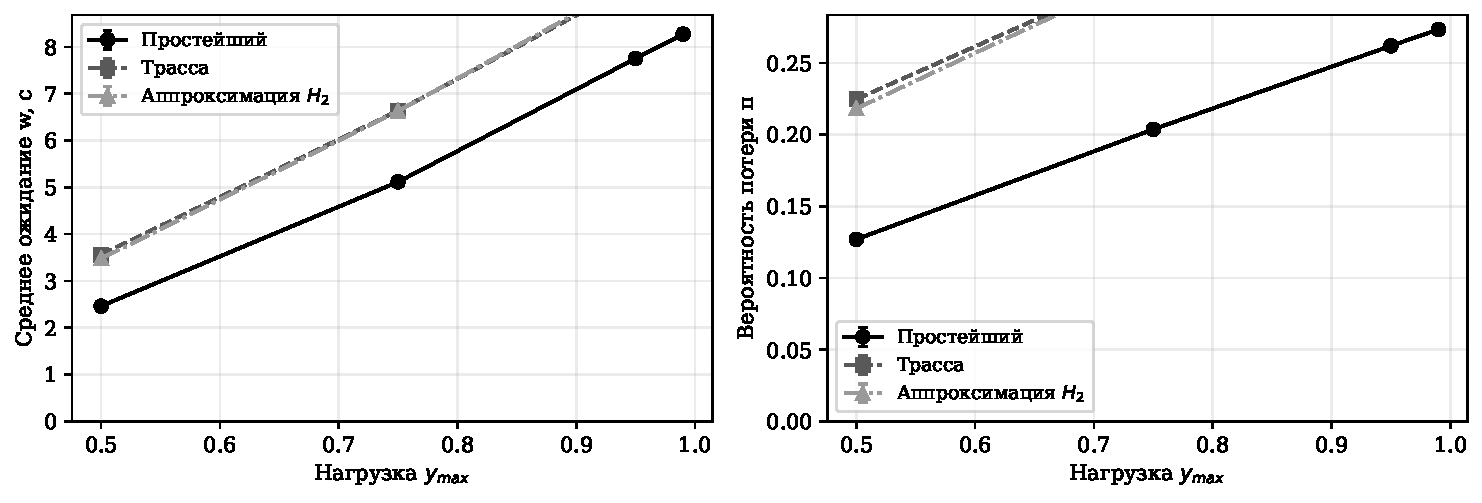
\includegraphics[width=\textwidth]{figures/arrival.pdf}\caption{Влияние входного потока на ожидание и потери при общем среднем интервале}\end{figure}

\begin{center}\small\renewcommand{\arraystretch}{1.3}
\begin{tabular}{|l|c|c|c|c|c|}\hline
Поток & \(y_{\max}\) & \(\pi\) & \(w\), с & \(u\), с & \(\overline\rho\)\\\hline
П & 0,50 & 0,1269 & 2,4629 & 11,3704 & 0,3237\\\hline
П & 0,75 & 0,2036 & 5,1160 & 18,4669 & 0,4425\\\hline
П & 0,95 & 0,2618 & 7,7534 & 24,6666 & 0,5197\\\hline
П & 0,99 & 0,2733 & 8,2744 & 25,8977 & 0,5330\\\hline
Т & 0,50 & 0,2246 & 3,5598 & 12,4633 & 0,2869\\\hline
Т & 0,75 & 0,3166 & 6,6387 & 19,9835 & 0,3790\\\hline
Т & 0,95 & 0,3741 & 9,3581 & 26,2496 & 0,4394\\\hline
Т & 0,99 & 0,3855 & 9,9401 & 27,5354 & 0,4493\\\hline
А & 0,50 & 0,2181 & 3,4766 & 12,3785 & 0,2880\\\hline
А & 0,75 & 0,3151 & 6,6291 & 19,9736 & 0,3782\\\hline
А & 0,95 & 0,3779 & 9,4170 & 26,3080 & 0,4347\\\hline
А & 0,99 & 0,3894 & 10,0014 & 27,6047 & 0,4447\\\hline
\end{tabular}\end{center}

\concl{При \(y_{\max}=0{,}95\) вероятность потери для Т равна 37,41\%, для А -- 37,79\%, для П -- 26,18\%. Большая вариация интервалов создаёт серии близких поступлений, которые заполняют небольшие накопители; длинные интервалы затем приводят к простоям. Поэтому при большей доле отказов фактическая загрузка может быть меньше.}

\subsection{Серия по фактической загрузке}
Для простейшего потока среднее \(b\) подбирается по уравнению
\begin{gather}
\frac13\sum_{j=1}^3(1-p_{0j}(b))=\rho_0,\qquad
p_{0j}(b)=\left(\sum_{k=0}^{K_j+E_j}(\lambda\alpha_jb)^k\right)^{-1},\\
\rho_0\in\{0{,}5;\,0{,}75;\,0{,}95;\,0{,}99\},\qquad \lambda=1/a.
\end{gather}
У П3 с \(E_2\) и без очереди вероятность занятости при простейшем входе зависит от среднего обслуживания; для этого прибора та же формула применяется при вместимости один. Подобранное \(b\) затем сохраняется при замене входа на Т и А. Выполнено по восемь повторений и 200000 прошедших заявок.

\begin{center}\small\renewcommand{\arraystretch}{1.3}
\begin{tabular}{|l|c|c|c|c|}\hline
\(\rho_0\) & \(b\), с & Поток П & Трасса Т & Аппрокс. А\\\hline
0,50 & 15,964 & 0,4999 & 0,4241 & 0,4220\\\hline
0,75 & 36,678 & 0,7500 & 0,6365 & 0,6239\\\hline
0,95 & 196,528 & 0,9500 & 0,9083 & 0,9036\\\hline
0,99 & 1048,172 & 0,9901 & 0,9826 & 0,9814\\\hline
\end{tabular}\end{center}

\begin{figure}[H]\centering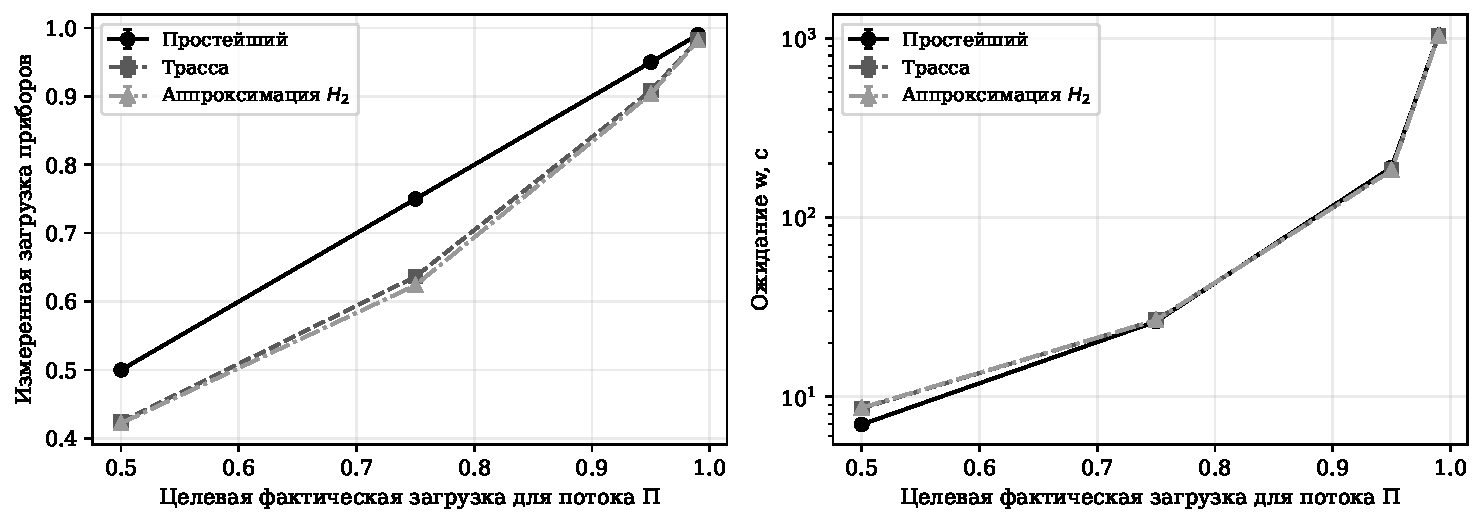
\includegraphics[width=\textwidth]{figures/actual_load.pdf}\caption{Измеренная загрузка и ожидание при калибровке по фактической загрузке простейшего потока}\end{figure}

\concl{Имитация воспроизводит заданную фактическую загрузку для потока П. При высокой загрузке малые накопители приводят к большому числу отказов. Для Т и А среднее обслуживание и средний вход сохраняются, а фактическая загрузка меняется из-за характера поступлений. Показаны оба способа задания нагрузки; они не смешиваются при сравнении.}

\subsection{Законы обслуживания}
Для оценки влияния обслуживания в этой серии один и тот же закон применяется ко всем трём приборам. Среднее \(b\) для одной нагрузки сохраняется. Рассматриваются
\begin{gather}
M:\quad B=-b\ln U,\qquad \nu_b=1,\\
E_2:\quad B=-\frac b2(\ln U_1+\ln U_2),\qquad \nu_b=\frac1{\sqrt2},\\
H_2:\quad B=\begin{cases}-\dfrac b{2q_b}\ln U_2,&U_1\leq q_b,\\
-\dfrac b{2(1-q_b)}\ln U_2,&U_1>q_b,\end{cases}
\quad q_b=\frac12\left(1+\sqrt{\frac35}\right),\quad \nu_b=2.
\end{gather}
Равномерные величины \(U,U_1,U_2\) независимы и лежат в \((0,1)\).

\begin{figure}[H]\centering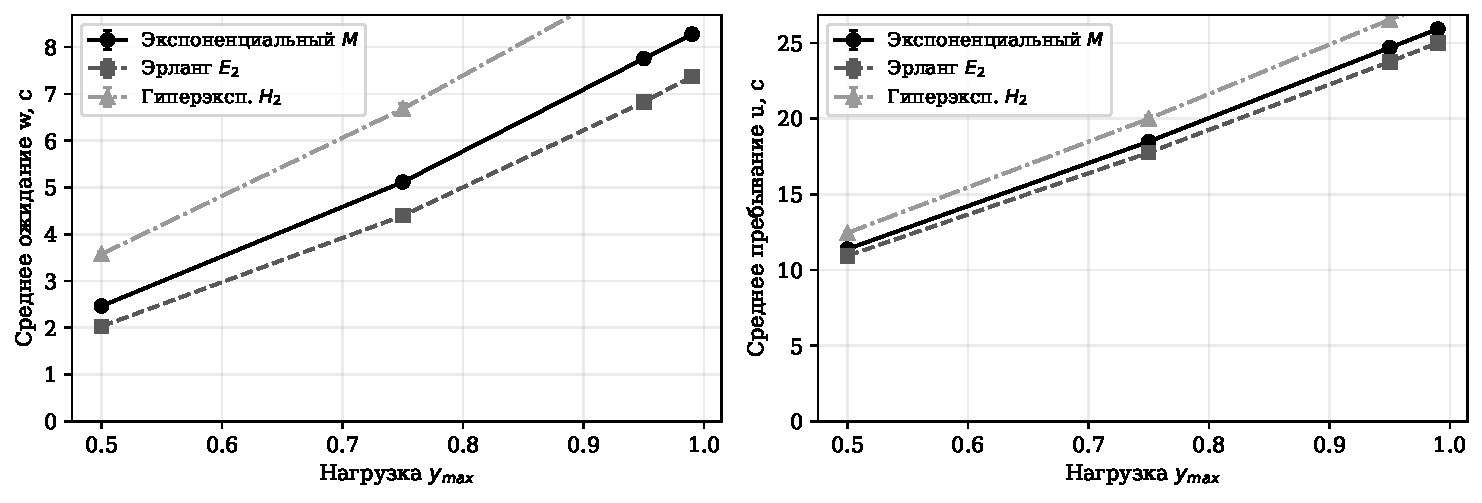
\includegraphics[width=\textwidth]{figures/service.pdf}\caption{Влияние закона обслуживания при сохранении среднего}\end{figure}

\concl{Рост вариации обслуживания увеличивает ожидание и пребывание. Редкие длительные обслуживания \(H_2\) надолго занимают прибор и усиливают очередь. Сумма двух фаз \(E_2\) имеет меньшую вариацию и даёт более ровное обслуживание. Влияние входного потока и обслуживания сравнивается при одинаковых средних; ранжирование относится к исследованным нагрузкам и структуре.}
\begin{center}\small\renewcommand{\arraystretch}{1.3}
\resizebox{\textwidth}{!}{\begin{tabular}{|l|c|c|c|c|}\hline
\(y_{\max}\) & \shortstack{Изменение \(w\), \%\\поток П \(\to\) А} & \shortstack{Изменение \(w\), \%\\обсл. \(M\) \(\to\) \(H_2\)} & \shortstack{Изменение \(\pi\), \%\\поток П \(\to\) А} & \shortstack{Изменение \(\pi\), \%\\обсл. \(M\) \(\to\) \(H_2\)}\\\hline
0,50 & 41,2 & 45,1 & 71,8 & 21,8\\\hline
0,95 & 21,5 & 22,9 & 44,3 & 14,6\\\hline
\end{tabular}}\end{center}

Проценты в этой таблице рассчитаны относительно базового варианта П или \(M\). Сравниваются выбранные изменения вариации: \(\nu_a=1\to2{,}812075\) и \(\nu_b=1\to2\); их величины различаются. Поэтому таблица характеризует данные эксперименты и не задаёт универсального ранжирования влияния потока и обслуживания.

\section{Длительность переходного процесса в системе}
Согласно методичке длительность переходного процесса измеряется количеством заявок, прошедших через систему от начала работы до вхождения в установившийся режим. Модель запускается из пустого состояния. Счётчик \(N\) увеличивается при завершении обслуживания или отказе; остановка совпадает по смыслу с \texttt{TERMINATE 1}. Число прошедших заявок в одном прогоне изменяется по сетке
\begin{equation}
N=10,20,50,100,200,300,600,1000,3000,10000,30000,100000.
\end{equation}
Выполнены 12 независимых повторений для пяти нагрузок \(y_{\max}=0{,}1;0{,}3;0{,}5;0{,}7;0{,}9\) и трёх потоков Т, А, П. По п. 2.2.2 задания нагрузка изменяется двумя способами: (а) изменением \(b\) при \(a=8{,}020778\) с; (б) изменением \(a\) при \(b=5\) с. Маршрутизация, накопители и законы обслуживания \((M,M,E_2)\) сохраняются.

В форме 2 ниже приведены срезы при \(y_{\max}=0{,}9\), способ (а). Строка «Заявок» содержит суммарное число прошедших заявок в 12 независимых прогонах: \(N_\Sigma=12N\). «Потери» -- целое суммарное число отказов. Средние времена и СКО вычислены по объединённым наблюдениям, длина очереди и загрузка -- по суммарным временным интегралам. Полные 360 строк для всех нагрузок, потоков и обоих способов сохранены в \texttt{results/gpss/form2.csv}.

Определения столбцов сохранены из методички: П(\%) -- относительное отличие вероятности потери от предыдущей строки; О(\%) -- такое же отличие среднего ожидания; Д(\%) -- отношение доверительного полуинтервала к среднему ожиданию. В П(\%) и О(\%) знаменатель -- текущее значение, как в числовом примере формы 2 на с. 7 задания. При нулевом текущем значении отношение не определено и обозначено прочерком.
\begin{gather}
\text{П}(\%)=\frac{|\pi_N-\pi_{N_{\text{пред}}}|}{|\pi_N|}\,100\%,\qquad
\text{О}(\%)=\frac{|w_N-w_{N_{\text{пред}}}|}{|w_N|}\,100\%,\\
\text{Д}(\%)=\frac{\varepsilon_w}{w_N}\,100\%,\qquad
I_w=[w_N-\varepsilon_w;\,w_N+\varepsilon_w].
\end{gather}
\Needspace{10\baselineskip}
Уровень доверия равен 0,95. Чтобы не считать зависимые ожидания независимыми, полуинтервал для отношения сумм оценивается по 12 независимым прогонам. Если \(S_r=\sum_i W_{ri}\), \(n_r\) -- число зарегистрированных ожиданий в прогоне, то
\begin{equation}
w_N=\frac{\sum_r S_r}{\sum_r n_r},\qquad
\varepsilon_w=t_{0{,}975;R-1}\,
\frac{\sqrt{\dfrac{R}{R-1}\sum_{r=1}^R(S_r-w_N n_r)^2}}{\sum_{r=1}^R n_r}
+\Delta_{\text{окр}},\qquad R=12.
\end{equation}
К полученному полуинтервалу добавляется допуск округления среднего 0,0005 с. Это приближённый интервал по независимым повторениям (дельта-метод). При малых \(N\) он служит оценкой разброса, а не подтверждением стационарности.

\noindent\begin{minipage}{\textwidth}\noindent\hfill Форма 2\par\begin{center}\textbf{Результаты имитационных экспериментов}\end{center}
\begin{center}\small\renewcommand{\arraystretch}{1.25}
\resizebox{\textwidth}{!}{\begin{tabular}{|r|r|c|c|c|c|c|c|c|c|c|}
\cline{1-8}
\multicolumn{2}{|c|}{Исх. данные} & \(K\) & \(E\) & поток & \(a\) & \(b\) & КВ & \multicolumn{3}{l}{}\\\cline{1-8}
\multicolumn{2}{|c|}{GPSS, Т} & 3 & \((2,1,0)\) & трасса & 8,0208 & 16,0416 & \((1;1;\frac1{\sqrt2})\) & \multicolumn{3}{l}{}\\\hline
Заявок & \shortstack{Поте-\\ри} & \shortstack{Вер-ть\\потери} & П(\%) & \shortstack{Длина\\очер.} & \shortstack{Загру-\\зка} & \shortstack{Ср.вр.\\ож.} & О(\%) & \shortstack{СКО\\вр.ож.} & \shortstack{Дов.\\инт.} & Д(\%)\\\hline
120 & 35 & 0,2917 & -- & 0,745 & 0,560 & 6,529 & -- & 12,459 & \(\pm 2,649\) & 40,6\\\hline
240 & 86 & 0,3583 & 18,6 & 0,549 & 0,409 & 4,753 & 37,4 & 9,932 & \(\pm 1,435\) & 30,2\\\hline
600 & 195 & 0,3250 & 10,3 & 0,683 & 0,467 & 6,552 & 27,5 & 13,432 & \(\pm 1,581\) & 24,1\\\hline
1200 & 441 & 0,3675 & 11,6 & 0,675 & 0,421 & 7,941 & 17,5 & 15,088 & \(\pm 0,904\) & 11,4\\\hline
2400 & 944 & 0,3933 & 6,6 & 0,760 & 0,470 & 8,271 & 4,0 & 14,706 & \(\pm 0,841\) & 10,2\\\hline
3600 & 1305 & 0,3625 & 8,5 & 0,664 & 0,426 & 8,216 & 0,7 & 16,156 & \(\pm 0,866\) & 10,5\\\hline
7200 & 2622 & 0,3642 & 0,5 & 0,689 & 0,431 & 8,626 & 4,7 & 16,770 & \(\pm 0,616\) & 7,1\\\hline
12000 & 4384 & 0,3653 & 0,3 & 0,703 & 0,433 & 8,816 & 2,2 & 16,530 & \(\pm 0,493\) & 5,6\\\hline
36000 & 12991 & 0,3609 & 1,2 & 0,686 & 0,428 & 8,586 & 2,7 & 15,935 & \(\pm 0,315\) & 3,7\\\hline
120000 & 43516 & 0,3626 & 0,5 & 0,683 & 0,424 & 8,586 & 0,0 & 15,851 & \(\pm 0,182\) & 2,1\\\hline
360000 & 130226 & 0,3617 & 0,2 & 0,688 & 0,426 & 8,645 & 0,7 & 15,878 & \(\pm 0,122\) & 1,4\\\hline
1200000 & 433705 & 0,3614 & 0,1 & 0,689 & 0,425 & 8,654 & 0,1 & 15,898 & \(\pm 0,047\) & 0,5\\\hline
\end{tabular}}\end{center}
\end{minipage}\par\medskip
\noindent\begin{minipage}{\textwidth}\noindent\hfill Форма 2\par\begin{center}\textbf{Результаты имитационных экспериментов}\end{center}
\begin{center}\small\renewcommand{\arraystretch}{1.25}
\resizebox{\textwidth}{!}{\begin{tabular}{|r|r|c|c|c|c|c|c|c|c|c|}
\cline{1-8}
\multicolumn{2}{|c|}{Исх. данные} & \(K\) & \(E\) & поток & \(a\) & \(b\) & КВ & \multicolumn{3}{l}{}\\\cline{1-8}
\multicolumn{2}{|c|}{GPSS, А} & 3 & \((2,1,0)\) & аппр. & 8,0208 & 16,0416 & \((1;1;\frac1{\sqrt2})\) & \multicolumn{3}{l}{}\\\hline
Заявок & \shortstack{Поте-\\ри} & \shortstack{Вер-ть\\потери} & П(\%) & \shortstack{Длина\\очер.} & \shortstack{Загру-\\зка} & \shortstack{Ср.вр.\\ож.} & О(\%) & \shortstack{СКО\\вр.ож.} & \shortstack{Дов.\\инт.} & Д(\%)\\\hline
120 & 44 & 0,3667 & -- & 0,367 & 0,305 & 4,455 & -- & 10,268 & \(\pm 1,724\) & 38,7\\\hline
240 & 84 & 0,3500 & 4,8 & 0,361 & 0,324 & 4,573 & 2,6 & 9,881 & \(\pm 1,122\) & 24,5\\\hline
600 & 201 & 0,3350 & 4,5 & 0,542 & 0,379 & 6,137 & 25,5 & 12,659 & \(\pm 1,411\) & 23,0\\\hline
1200 & 400 & 0,3333 & 0,5 & 0,559 & 0,387 & 6,995 & 12,3 & 13,401 & \(\pm 1,106\) & 15,8\\\hline
2400 & 844 & 0,3517 & 5,2 & 0,656 & 0,410 & 8,163 & 14,3 & 15,395 & \(\pm 1,045\) & 12,8\\\hline
3600 & 1267 & 0,3519 & 0,1 & 0,702 & 0,423 & 8,748 & 6,7 & 16,228 & \(\pm 0,582\) & 6,6\\\hline
7200 & 2607 & 0,3621 & 2,8 & 0,717 & 0,426 & 8,999 & 2,8 & 16,738 & \(\pm 0,548\) & 6,1\\\hline
12000 & 4403 & 0,3669 & 1,3 & 0,706 & 0,424 & 9,026 & 0,3 & 16,583 & \(\pm 0,399\) & 4,4\\\hline
36000 & 13039 & 0,3622 & 1,3 & 0,697 & 0,429 & 8,702 & 3,7 & 15,735 & \(\pm 0,241\) & 2,8\\\hline
120000 & 43571 & 0,3631 & 0,2 & 0,688 & 0,425 & 8,637 & 0,8 & 15,846 & \(\pm 0,198\) & 2,3\\\hline
360000 & 131136 & 0,3643 & 0,3 & 0,692 & 0,424 & 8,732 & 1,1 & 15,998 & \(\pm 0,133\) & 1,5\\\hline
1200000 & 435892 & 0,3632 & 0,3 & 0,689 & 0,423 & 8,710 & 0,2 & 15,948 & \(\pm 0,048\) & 0,6\\\hline
\end{tabular}}\end{center}
\end{minipage}\par\medskip
\noindent\begin{minipage}{\textwidth}\noindent\hfill Форма 2\par\begin{center}\textbf{Результаты имитационных экспериментов}\end{center}
\begin{center}\small\renewcommand{\arraystretch}{1.25}
\resizebox{\textwidth}{!}{\begin{tabular}{|r|r|c|c|c|c|c|c|c|c|c|}
\cline{1-8}
\multicolumn{2}{|c|}{Исх. данные} & \(K\) & \(E\) & поток & \(a\) & \(b\) & КВ & \multicolumn{3}{l}{}\\\cline{1-8}
\multicolumn{2}{|c|}{GPSS, П} & 3 & \((2,1,0)\) & прост. & 8,0208 & 16,0416 & \((1;1;\frac1{\sqrt2})\) & \multicolumn{3}{l}{}\\\hline
Заявок & \shortstack{Поте-\\ри} & \shortstack{Вер-ть\\потери} & П(\%) & \shortstack{Длина\\очер.} & \shortstack{Загру-\\зка} & \shortstack{Ср.вр.\\ож.} & О(\%) & \shortstack{СКО\\вр.ож.} & \shortstack{Дов.\\инт.} & Д(\%)\\\hline
120 & 33 & 0,2750 & -- & 0,387 & 0,413 & 3,010 & -- & 7,960 & \(\pm 1,622\) & 53,9\\\hline
240 & 63 & 0,2625 & 4,8 & 0,447 & 0,463 & 3,903 & 22,9 & 9,912 & \(\pm 1,377\) & 35,3\\\hline
600 & 144 & 0,2400 & 9,4 & 0,584 & 0,479 & 5,907 & 33,9 & 12,998 & \(\pm 1,781\) & 30,2\\\hline
1200 & 279 & 0,2325 & 3,2 & 0,624 & 0,490 & 6,536 & 9,6 & 14,231 & \(\pm 1,162\) & 17,8\\\hline
2400 & 599 & 0,2496 & 6,8 & 0,722 & 0,506 & 7,564 & 13,6 & 15,852 & \(\pm 1,097\) & 14,5\\\hline
3600 & 889 & 0,2469 & 1,1 & 0,695 & 0,501 & 7,403 & 2,2 & 15,700 & \(\pm 0,889\) & 12,0\\\hline
7200 & 1766 & 0,2453 & 0,7 & 0,687 & 0,503 & 7,394 & 0,1 & 15,310 & \(\pm 0,555\) & 7,5\\\hline
12000 & 2979 & 0,2482 & 1,2 & 0,688 & 0,505 & 7,369 & 0,3 & 15,160 & \(\pm 0,555\) & 7,5\\\hline
36000 & 8884 & 0,2468 & 0,6 & 0,653 & 0,501 & 6,972 & 5,7 & 14,270 & \(\pm 0,188\) & 2,7\\\hline
120000 & 29608 & 0,2467 & 0,0 & 0,659 & 0,501 & 7,026 & 0,8 & 14,416 & \(\pm 0,145\) & 2,1\\\hline
360000 & 89291 & 0,2480 & 0,5 & 0,659 & 0,502 & 7,038 & 0,2 & 14,448 & \(\pm 0,090\) & 1,3\\\hline
1200000 & 297117 & 0,2476 & 0,2 & 0,660 & 0,501 & 7,031 & 0,1 & 14,455 & \(\pm 0,044\) & 0,6\\\hline
\end{tabular}}\end{center}
\end{minipage}\par\medskip
На графиках показаны объединённые оценки 12 независимых повторений в зависимости от числа прошедших заявок \(N\) \textit{в одном прогоне}.
\begin{figure}[H]\centering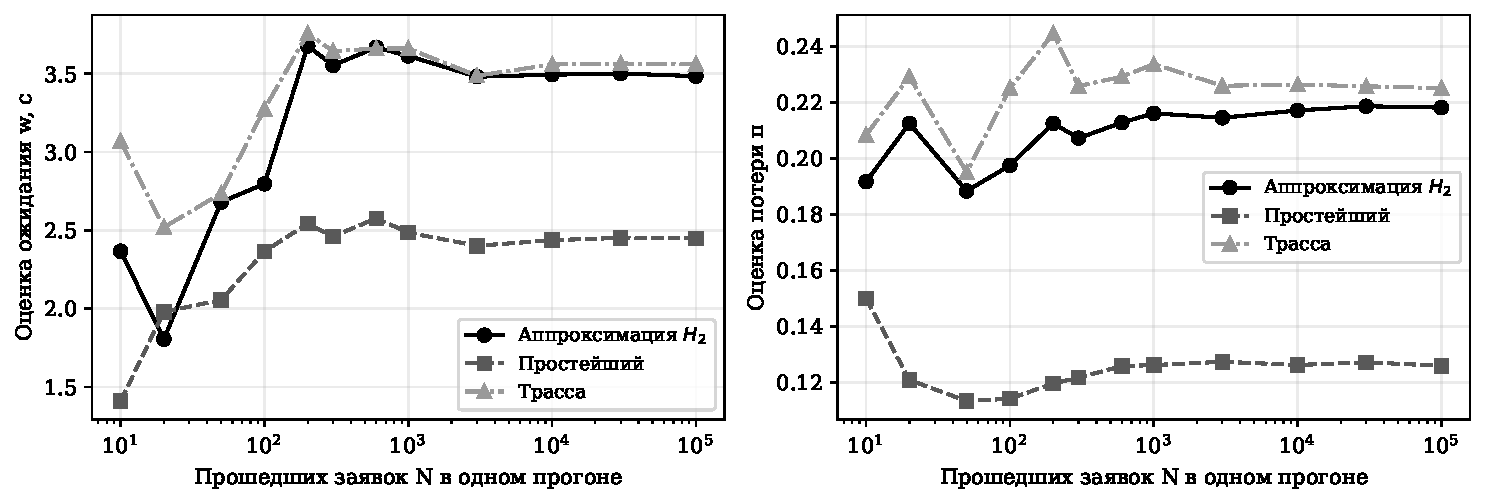
\includegraphics[width=\textwidth]{figures/transient_50.pdf}\caption{Изменение оценок при увеличении числа прошедших заявок, нагрузка 0,5}\end{figure}

\begin{figure}[H]\centering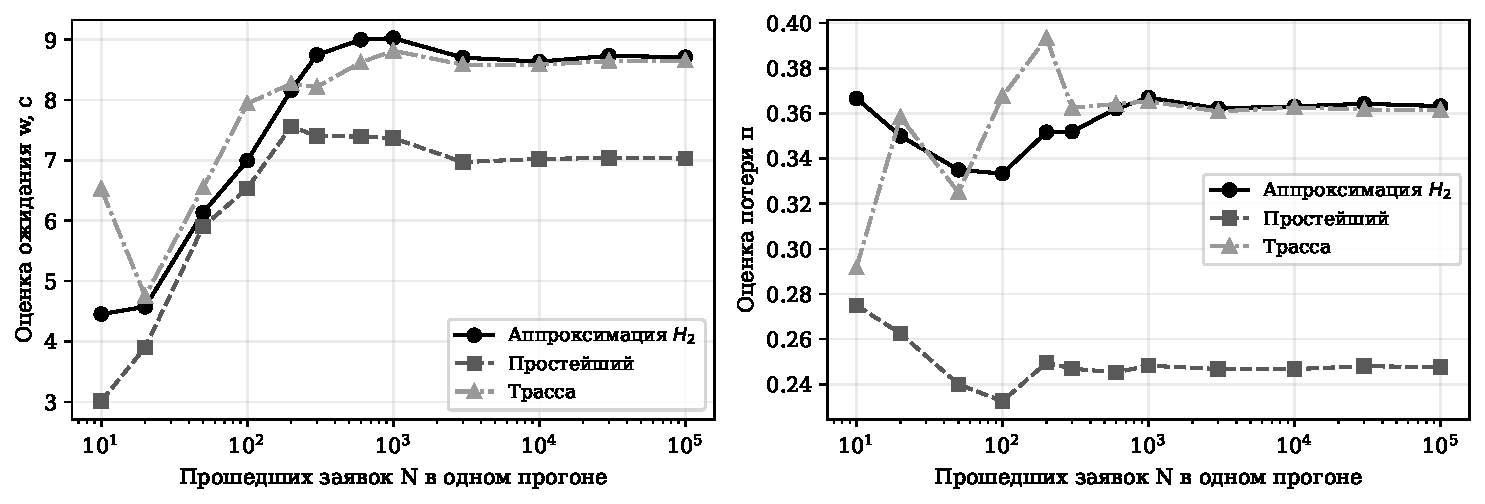
\includegraphics[width=\textwidth]{figures/transient_90.pdf}\caption{Изменение оценок при увеличении числа прошедших заявок, нагрузка 0,9}\end{figure}


Для воспроизводимой оценки устойчивости выбран порог 5\%. Начиная с \(N_{\text{уст}}\), на всех оставшихся точках сетки отклонения средних \(w\) и \(\pi\) от оценок при \(N=100000\) должны быть меньше 5\%, а Д(\%) -- меньше 5\%. Порог 5\% и сетка -- выбор исследователя; методичка не задаёт их численно. В таблице приведены первые подходящие точки сетки; прочерк означает, что критерий на исследованной сетке не выполнен.

\begin{center}\small\renewcommand{\arraystretch}{1.3}
\resizebox{\textwidth}{!}{\begin{tabular}{|l|c|c|c|c|c|c|}\hline
Изменяется & Поток & 0,1 & 0,3 & 0,5 & 0,7 & 0,9\\\hline
\(b\) & Т & 3000 & 3000 & 3000 & 3000 & 3000\\\hline
\(b\) & А & 10000 & 3000 & 3000 & 3000 & 1000\\\hline
\(b\) & П & 30000 & 3000 & 3000 & 3000 & 3000\\\hline
\(a\) & Т & 3000 & 3000 & 3000 & 3000 & 3000\\\hline
\(a\) & А & 10000 & 3000 & 3000 & 3000 & 1000\\\hline
\(a\) & П & 10000 & 3000 & 3000 & 3000 & 3000\\\hline
\end{tabular}}\end{center}

\begin{figure}[H]\centering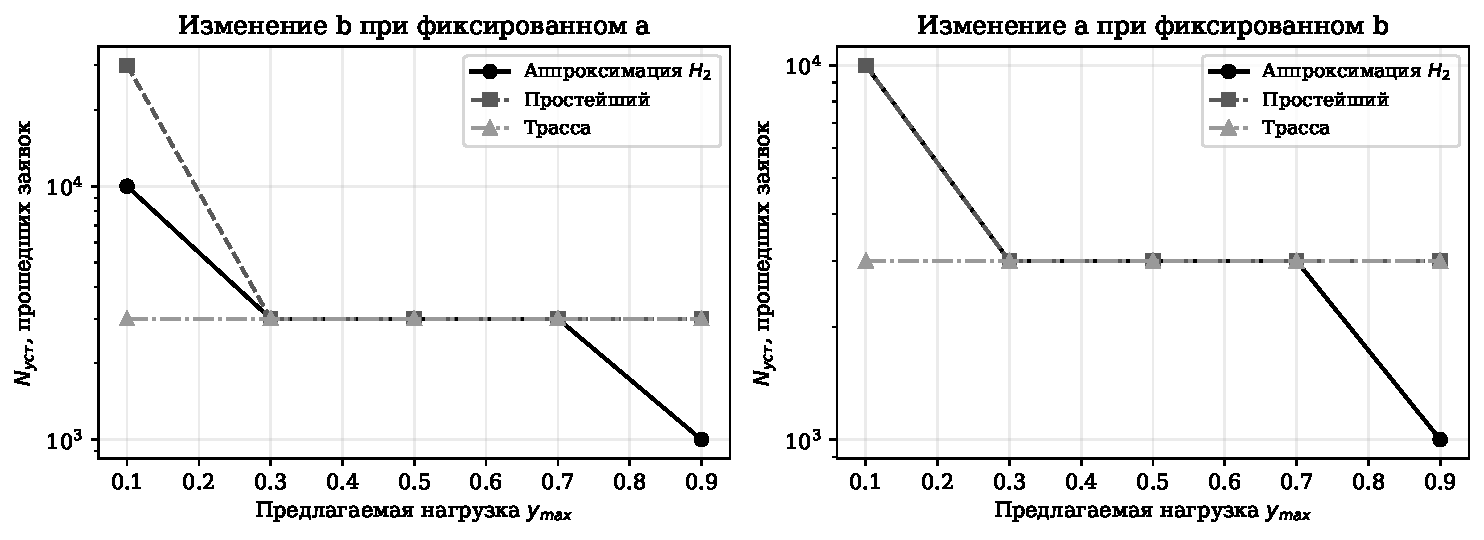
\includegraphics[width=\textwidth]{figures/transient_loads.pdf}\caption{Длительность переходного процесса по принятому критерию для пяти нагрузок}\end{figure}


\concl{При одинаковом отношении \(b/a\) и тех же потоках случайных чисел меняется только масштаб времени. В опытах с изменением \(a\) все интервалы трассы умножаются на \(a/a_{\text{УИР1}}\), порядок и коэффициент вариации сохраняются. В обязательной серии Т/А/П среднее \(a\) остаётся исходным. При малой нагрузке ожидания редки, поэтому их относительная погрешность может оставаться большой даже при быстром выходе системы на стационарный режим. Оценка \(N_{\text{уст}}\) объединяет переходный процесс и статистическую погрешность. Для трассы устойчивость оценок не означает независимость повторяемых интервалов. В основных стационарных сериях отброшены первые 10000 прошедших заявок; точность оценивается отдельно по интервалам независимых повторений.}

\Needspace{13\baselineskip}
\section{Ёмкость накопителей и число приборов}
Для анализа буфера во всех трёх накопителях устанавливается одна ёмкость \(E\). Другие параметры сохраняются. Это семейство включает исходную маршрутизацию и законы \(M/M/E_2\), но изменяет ёмкости исходной СМО 2/1/0.

\begin{figure}[H]\centering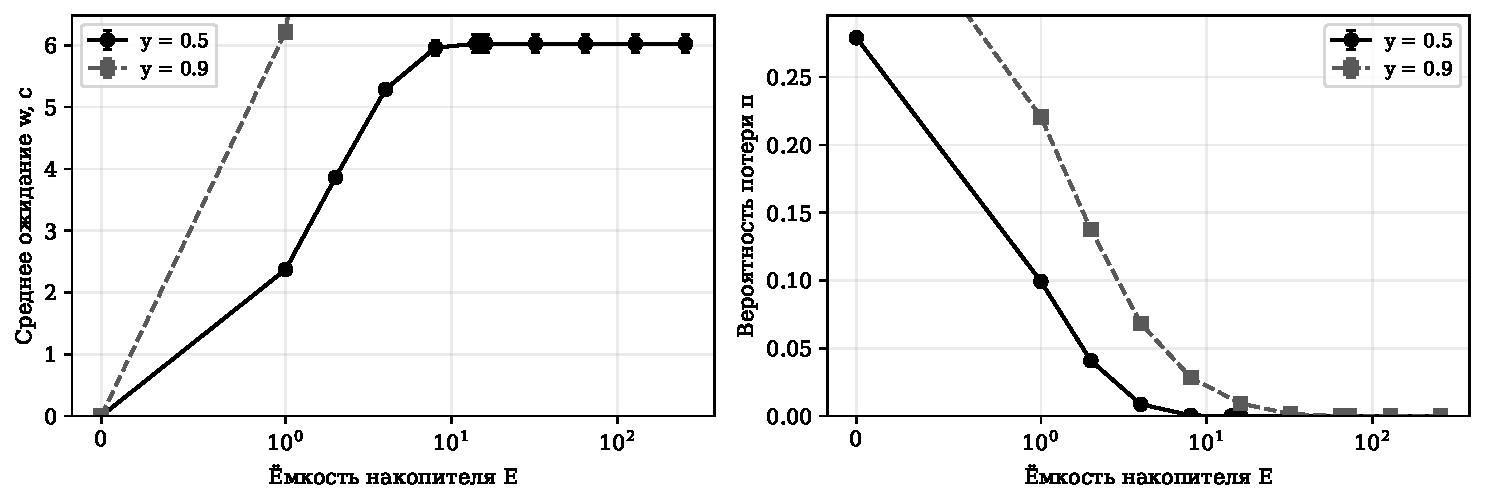
\includegraphics[width=\textwidth]{figures/buffer.pdf}\caption{Зависимость ожидания и потерь от ёмкости каждого накопителя}\end{figure}

\begin{center}\small\renewcommand{\arraystretch}{1.3}
\begin{tabular}{|l|c|c|c|}\hline
\(y_{\max}\) & \(E^*_{\text{набл}}\) & Потери при \(E^*-1\) & Потери при \(E^*\)\\\hline
0,50 & 15 & 1 & 0\\\hline
0,90 & 72 & 1 & 0\\\hline
\end{tabular}\end{center}


Для определения минимальной наблюдаемой ёмкости сначала выполнены опыты по сетке ёмкостей и с практически неограниченным накопителем. Затем уточнена граница и отдельно проверены \(E^*-1\) и \(E^*\) на тех же восьми наборах начальных чисел генераторов. В каждой проверке зарегистрировано 480000 прошедших заявок после разгона.

\concl{В таблице приведены границы отсутствия потерь в выполненной серии. При бесконечном времени наблюдения конечный буфер системы с экспоненциальными интервалами всё равно имеет ненулевую вероятность потери. Поэтому термин «неограниченный накопитель» здесь означает достаточность для точности и горизонта проведённого опыта. Увеличение буфера снижает отказы, но позволяет большему числу заявок ожидать обслуживания.}

В отдельной серии число приборов \(K_j\) каждого из трёх узлов изменяется от 1 до 3. Всего система содержит 3, 6 или 9 приборов; это не изменение числа маршрутов. Выполнены два сравнения -- при неизменных \(a,b\) и при увеличении \(b\) в \(K_j\) раз, сохраняющем предлагаемую нагрузку на один прибор.

\begin{figure}[H]\centering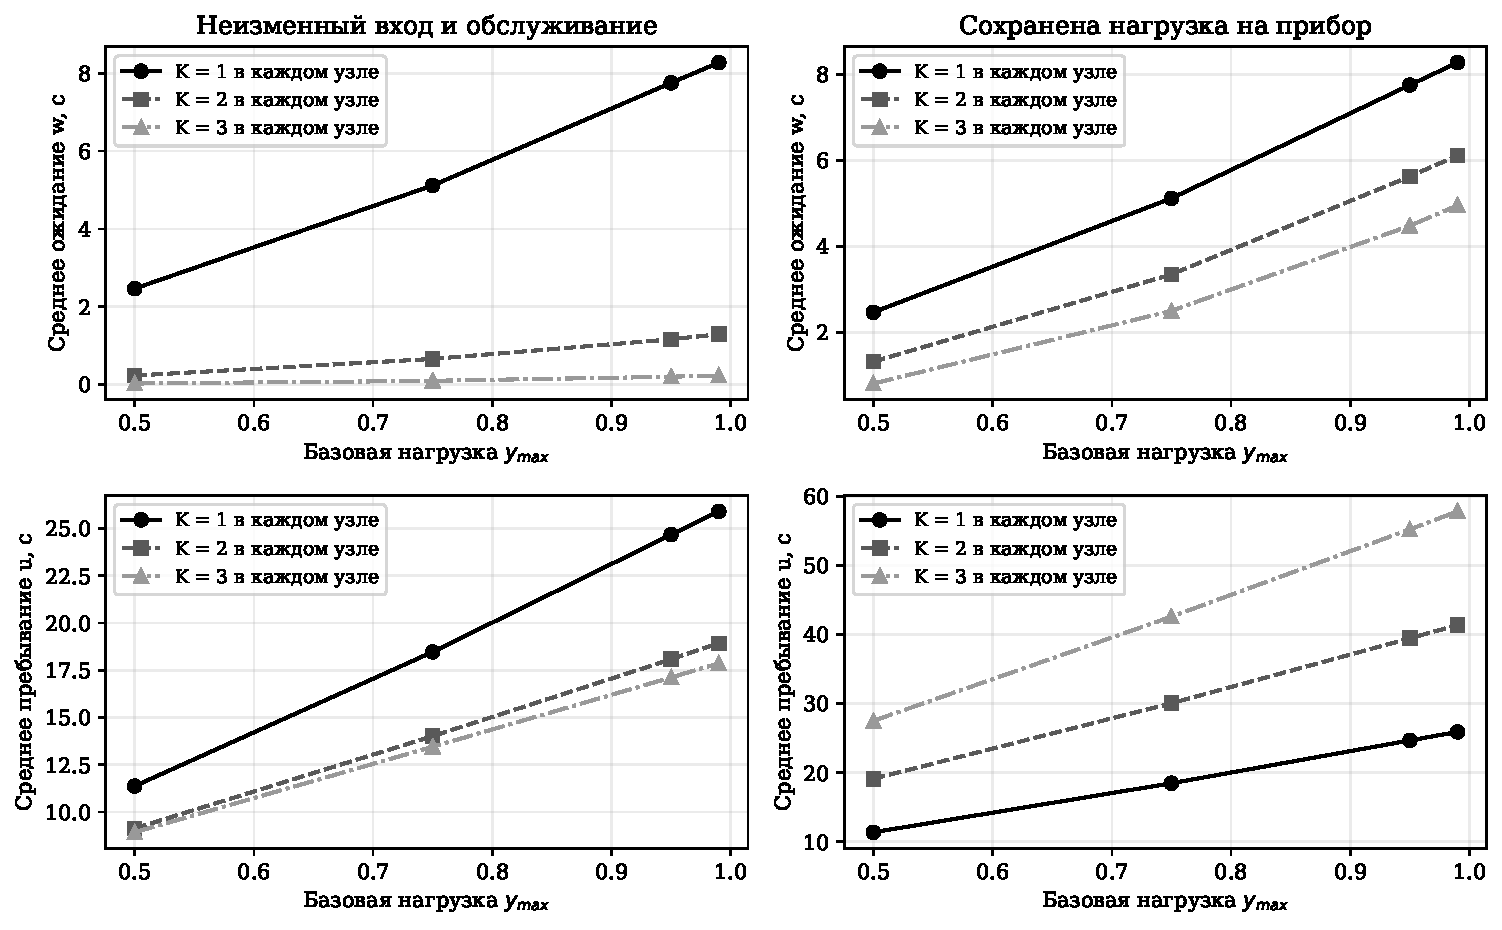
\includegraphics[width=\textwidth]{figures/servers.pdf}\caption{Влияние числа приборов в каждом из трёх узлов}\end{figure}


\section{Проверка по формулам M/M/1 и M/G/1}
Независимый проверочный опыт проводится для одного прибора с практически неограниченным накопителем, \(a=8\;\text{с}\), \(b=4\;\text{с}\), \(\rho=b/a=0{,}5\). Формулы бесконечного накопителя применяются только к этому проверочному опыту.
\begin{equation}
w_{M/G/1}=\frac{\lambda\operatorname{E}[B^2]}{2(1-\rho)}
=\frac{\rho b(1+\nu_b^2)}{2(1-\rho)},\qquad u=w+b.
\end{equation}
Для \(M/M/1\) при \(\nu_b=1\) получаем \(w=\rho b/(1-\rho)\).

\begin{center}\small\renewcommand{\arraystretch}{1.3}
\begin{tabular}{|l|c|c|c|}\hline
Закон & \(w_{\text{теор}}\), с & \(\overline w\), с & Дов. полуинт.\\\hline
\(M\) & 4,0000 & 3,9877 & \(\pm 0,0226\)\\\hline
\(E_2\) & 3,0000 & 2,9915 & \(\pm 0,0181\)\\\hline
\(H_2\) & 10,0000 & 10,1098 & \(\pm 0,1257\)\\\hline
\end{tabular}\end{center}


\concl{Во всех трёх случаях теоретическое значение попало в интервал повторений. Формула M/G/1 показывает прямое влияние второго момента обслуживания на ожидание; при том же среднем переход от \(E_2\) к \(H_2\) увеличивает теоретическое ожидание с 3 до 10 с.}

\Needspace{10\baselineskip}
\section{Распределения времени ожидания и пребывания СМО}
Таблицы GPSS сохраняют моменты и частоты \(W_i,U_i\). Коэффициент вариации -- отношение СКО к среднему. GPSS вычисляет исправленную выборочную дисперсию с делением на \(n-1\). Для независимых наблюдений такая оценка дисперсии несмещённа; времена ожидания одного прогона могут быть зависимыми, поэтому точность среднего оценивается по независимым повторениям. В таблице приведены средние оценки восьми повторений.
\begin{equation}
\widetilde\nu_w=\frac{\widetilde\sigma_w}{\widetilde w},\qquad
\widetilde\nu_u=\frac{\widetilde\sigma_u}{\widetilde u}.
\end{equation}

\begin{center}\small\renewcommand{\arraystretch}{1.3}
\resizebox{\textwidth}{!}{\begin{tabular}{|l|c|c|c|c|c|c|c|}\hline
Поток & \(y_{\max}\) & \(w\), с & \(\sigma_w\), с & \(\nu_w\) & \(u\), с & \(\sigma_u\), с & \(\nu_u\)\\\hline
П & 0,50 & 2,463 & 6,472 & 2,628 & 11,370 & 10,609 & 0,933\\\hline
П & 0,95 & 7,753 & 15,571 & 2,008 & 24,667 & 22,325 & 0,905\\\hline
Т & 0,50 & 3,560 & 7,690 & 2,160 & 12,463 & 11,406 & 0,915\\\hline
Т & 0,95 & 9,358 & 16,960 & 1,812 & 26,250 & 23,311 & 0,888\\\hline
А & 0,50 & 3,477 & 7,625 & 2,193 & 12,379 & 11,369 & 0,918\\\hline
А & 0,95 & 9,417 & 16,977 & 1,803 & 26,308 & 23,300 & 0,886\\\hline
\end{tabular}}\end{center}

\begin{figure}[H]\centering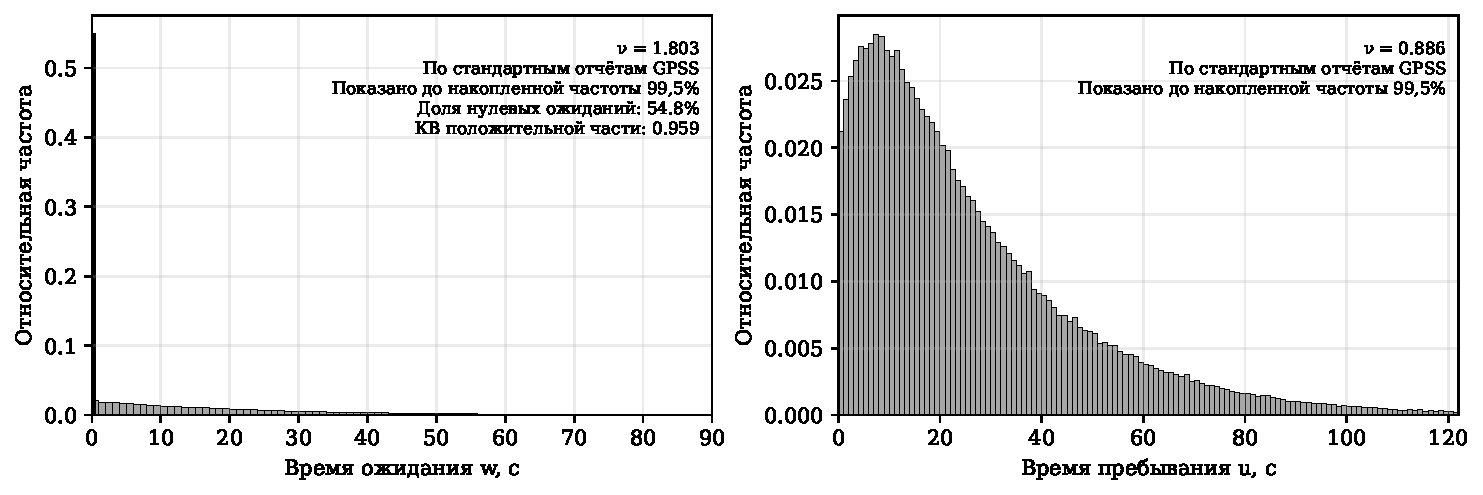
\includegraphics[width=\textwidth]{figures/hist_smo.pdf}\caption{Распределения ожидания и пребывания для потока А при нагрузке 0,95}\end{figure}

Для ожидания отдельно учитывается доля нулей \(p_0\). Дополнительная проверка формы положительной части использует эмпирические моменты:
\begin{equation}
\widetilde w_+=\frac{\widetilde w}{1-p_0},\qquad
\widetilde\nu_+^2=(1-p_0)\frac{\overline{W^2}}{\widetilde w^2}-1.
\end{equation}

Здесь \(p_0=0,548\), \(\nu_w=1,803\), \(\nu_+=0,959\). Для положительного ожидания выбирается экспоненциальная гипотеза, для пребывания (\(\nu_u=0,886\)) -- гипотеза Эрланга. Это аппроксимации по двум моментам; вид распределения однозначно не устанавливается.


\newpage
\begin{center}\textbf{Часть 2 «Исследование свойств сетей массового обслуживания (СеМО)»}\end{center}
\section{Сетевые модели. Вариант 6/6}
В соответствии с теоретическим материалом (п. 6.7.11) производительность сети обозначается \(\lambda_0\), среднее время пребывания в сети -- \(U\); \(w_j,u_j\) относятся к одному посещению узла. Сетевое ожидание \(W\) учитывает все посещения за цикл.
По строке 6 таблицы 1 задана модель М1 с тремя узлами, количеством приборов \(K=(1,4,1)\); изменяемый закон обслуживания назначается узлу У3. По строке 6 таблицы 2
\begin{equation}
p_{10}=0{,}2,\qquad p_{12}=0{,}3,\qquad
b_1=1\;\text{с},\quad b_2=15\;\text{с},\quad b_3=10\;\text{с}.
\end{equation}
Параметры \(p_{13}\) и \(b_4\) из той же строки используются для других типов моделей, на графе М1 они не задаются. Недостающая вероятность выбирается по условию суммы вероятностей исходящих дуг, равной единице.
\begin{equation}
p_{13}^{(M1)}=1-p_{10}-p_{12}=0{,}5,\qquad p_{21}=p_{31}=1.
\end{equation}
Все накопители сети неограниченны; обслуживание FIFO. В замкнутой сети условный узел «0» не содержит задержки, заявка возвращается в У1; число заявок \(M\) сохраняется. В разомкнутой сети «0» является внешним источником и стоком.
\begin{figure}[H]\centering
\begin{tikzpicture}[>=Stealth,node distance=3.5cm]
\node[draw,circle,minimum size=16mm] (one) {У1};
\node[draw,circle,minimum size=16mm,above right=9mm and 38mm of one] (two) {У2};
\node[draw,circle,minimum size=16mm,below right=9mm and 38mm of one] (three) {У3};
\draw[->] (one) to[bend left=12] node[above,sloped] {\(p_{12}=0{,}3\)} (two);
\draw[->] (two) to[bend left=12] node[pos=.3,below,sloped] {1} (one);
\draw[->] (one) to[bend right=12] node[below,sloped] {\(p_{13}=0{,}5\)} (three);
\draw[->] (three) to[bend right=12] node[pos=.3,above,sloped] {1} (one);
\draw[->] (one) to[out=140,in=220,looseness=7] node[left] {«0», \(p_{10}=0{,}2\)} (one);
\node[left=13mm of one,below=16mm] {\(K_1=1,\ b_1=1\)};
\node[right=8mm of two] {\(K_2=4,\ b_2=15\)};
\node[right=8mm of three] {\(K_3=1,\ b_3=10\)};
\end{tikzpicture}
\caption{Граф замкнутой сети М1. Средние длительности указаны в секундах}
\end{figure}
\begin{figure}[H]\centering
\begin{tikzpicture}[>=Stealth]
\node[draw,circle,minimum size=13mm] (one) at (0,0) {У1};
\node[draw,circle,minimum size=13mm] (two) at (4,1.15) {У2};
\node[draw,circle,minimum size=13mm] (three) at (4,-1.15) {У3};
\draw[->] (-3,0.35)--node[above] {вход \(\lambda_0\)} (one);
\draw[->] (one)--node[below] {выход \(0{,}2\)} (-3,-.55);
\draw[->] (one) to[bend left=12] node[above,sloped] {0,3} (two);
\draw[->] (two) to[bend left=12] (one);
\node[fill=white,inner sep=1pt] at (2.8,.45) {1};
\draw[->] (one) to[bend right=12] node[below,sloped] {0,5} (three);
\draw[->] (three) to[bend right=12] (one);
\node[fill=white,inner sep=1pt] at (2.8,-.45) {1};
\node[right=8mm of two] {\(K_2=4,\ b_2=15\)};
\node[right=8mm of three] {\(K_3=1,\ b_3=10\)};
\node[below=16mm of one] {\(K_1=1,\ b_1=1\)};
\end{tikzpicture}
\caption{Граф разомкнутой сети. Узловые параметры совпадают с замкнутой сетью}
\end{figure}
\subsection{Коэффициенты передач и предел производительности}
За один цикл принимается прохождение через «0». В разомкнутой сети это путь от входа до выхода. Коэффициент передачи \(\alpha_j\) равен среднему числу посещений У\(j\) за цикл.
\begin{equation}
\lambda_0=\frac{N_0}{T},\qquad \alpha_j=\frac{N_j}{N_0}.
\end{equation}
Здесь \(N_0\) -- число прохождений через нулевую точку за время \(T\); \(N_j\) -- число обслуживаний в узле. Теоретические коэффициенты передач и предел интенсивности для заданного графа:
\begin{gather}
\alpha_1=\frac1{p_{10}}=5,\qquad
\alpha_2=\frac{p_{12}}{p_{10}}=1{,}5,\qquad
\alpha_3=\frac{p_{13}}{p_{10}}=2{,}5,\\
\lambda_j=\alpha_j\lambda_0,\qquad
D_j=\alpha_j b_j,\qquad
\lambda_{0,\text{пред}}=\min_j\frac{K_j}{D_j}
=\min\left(\frac15;\frac4{22{,}5};\frac1{25}\right)
=0{,}04\;\text{с}^{-1}.
\end{gather}
Узкое место -- У3, имеющий наибольшую удельную потребность \(D_j/K_j\). Для открытой сети стационарный режим требует строгого неравенства \(\lambda_0<0{,}04\;\text{с}^{-1}\). При равенстве очередь У3 не имеет конечного стационарного среднего.

\section{Замкнутая сеть, насыщение и критическое число заявок}
Сначала все обслуживания экспоненциальны. Помимо событийной имитации используется независимый расчёт для экспоненциальной сети с многоканальными узлами.
\begin{gather}
g_j(0)=1,\qquad g_j(n)=g_j(n-1)\frac{\alpha_jb_j}{\min(n,K_j)},\\
G(M)=\sum_{n_1+n_2+n_3=M}\prod_{j=1}^3g_j(n_j),\qquad
P(n_1,n_2,n_3)=\frac{\prod_jg_j(n_j)}{G(M)},\\
\lambda_0(M)=\frac{G(M-1)}{G(M)},\qquad
U(M)=\frac{M}{\lambda_0(M)},\qquad
W(M)=\frac{l_\Sigma(M)}{\lambda_0(M)}.
\end{gather}
Здесь \(G(M)\) -- нормирующая сумма сети; \(\lambda_0\) -- число завершённых циклов в секунду, то есть число прохождений через нулевую точку, делённое на время наблюдения. Узловые времена в сетевых суммах обозначены \(w_j,u_j\).

\begin{figure}[H]\centering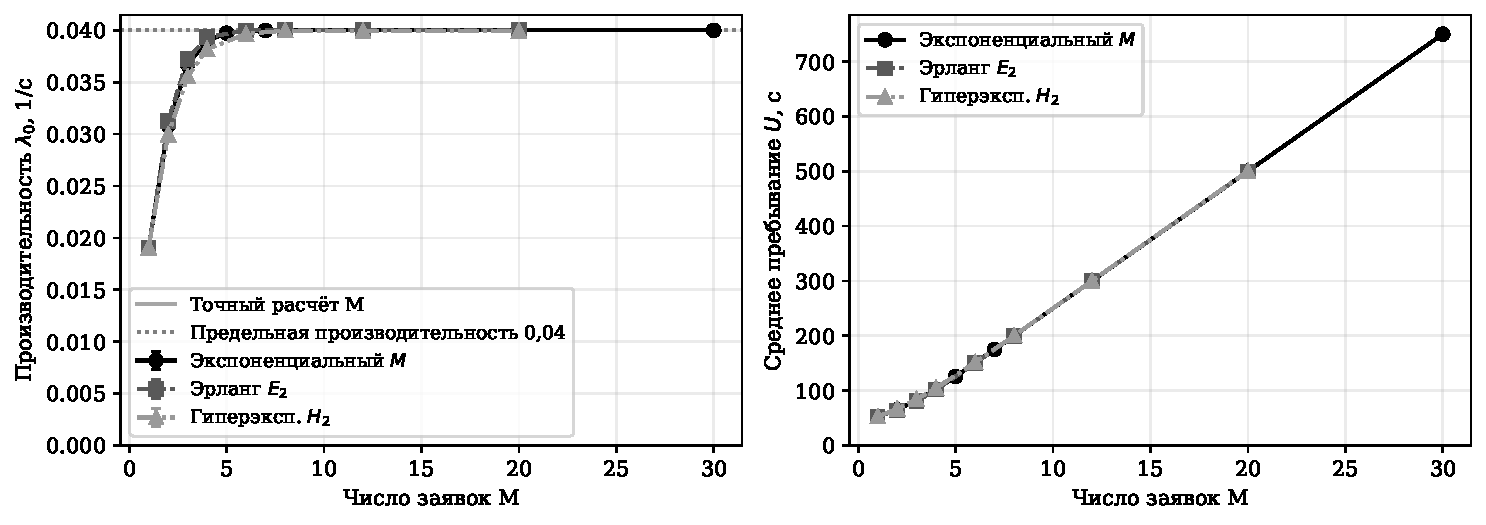
\includegraphics[width=\textwidth]{figures/closed.pdf}\caption{Зависимости производительности и пребывания от числа циркулирующих заявок}\end{figure}

\begin{center}\small\renewcommand{\arraystretch}{1.3}
\begin{tabular}{|l|c|c|c|}\hline
\(M\) & \(\lambda_{0,\text{точн}}\), с\(^{-1}\) & GPSS: \(\lambda_0\pm\varepsilon\), с\(^{-1}\) & Точный рост, \%\\\hline
1 & 0,019048 & 0,019061 \(\pm 0,000127\) & --\\\hline
2 & 0,030826 & 0,030866 \(\pm 0,000205\) & 61,835\\\hline
3 & 0,036682 & 0,036717 \(\pm 0,000244\) & 18,998\\\hline
4 & 0,038994 & 0,039015 \(\pm 0,000263\) & 6,304\\\hline
5 & 0,039720 & 0,039729 \(\pm 0,000269\) & 1,861\\\hline
6 & 0,039926 & 0,039927 \(\pm 0,000270\) & 0,519\\\hline
7 & 0,039981 & 0,039980 \(\pm 0,000270\) & 0,138\\\hline
8 & 0,039995 & 0,039994 \(\pm 0,000270\) & 0,035\\\hline
\end{tabular}\end{center}


Критическое число определяется по порогу 1\% относительного приращения при добавлении одной заявки. Условие проверено точным расчётом для всех последующих \(M\leq30\); имитационная серия GPSS содержит точки \(M=1,2,3,4,5,6,7,8,12,20,30\) для экспоненциальной сети. Точечные оценки GPSS имеют случайную погрешность, поэтому порог 1\% проверяется по точному контролю, а насыщение сопоставляется с имитационным графиком.
\begin{equation}
\frac{\lambda_0(M)-\lambda_0(M-1)}{\lambda_0(M-1)}<0{,}01
\quad\Longrightarrow\quad M^*=6.
\end{equation}
Это критерий выбранной точности; производительность математически продолжает приближаться к пределу. После насыщения дополнительная заявка в основном увеличивает очередь У3, поэтому \(U\approx M/0{,}04=25M\) растёт почти линейно.

\begin{figure}[H]\centering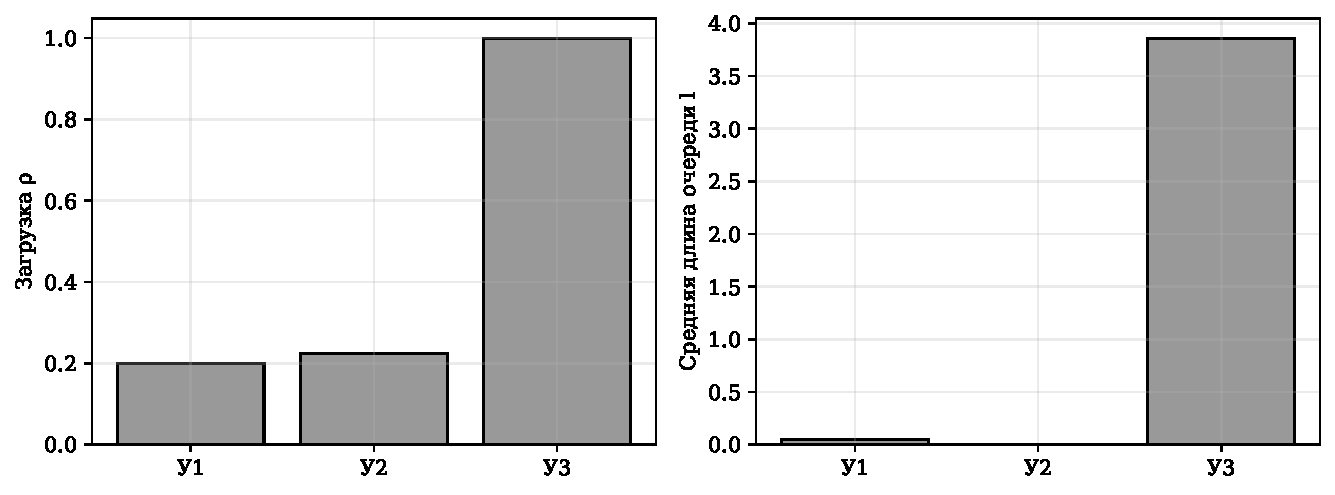
\includegraphics[width=\textwidth]{figures/node_bottleneck.pdf}\caption{Узловые загрузки и очереди экспоненциальной ЗСеМО при M = 6}\end{figure}


\subsection{Устранение узкого места}
При \(M=6\) отдельно проверяются ускорение У3 вдвое и добавление второго прибора У3.

\begin{figure}[H]\centering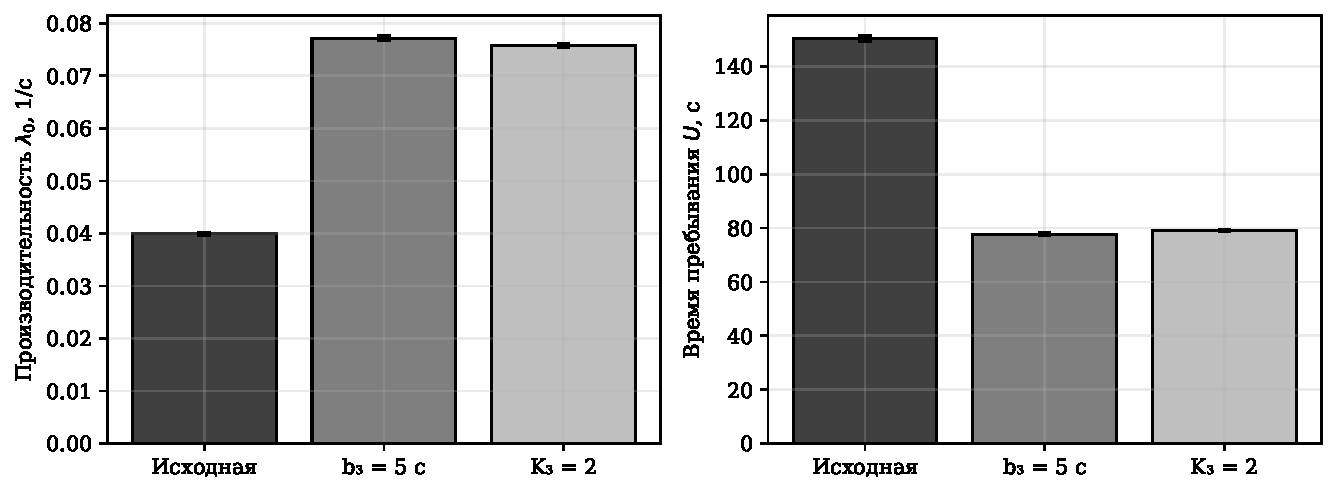
\includegraphics[width=\textwidth]{figures/bottleneck.pdf}\caption{Изменение сетевых характеристик после устранения узкого места}\end{figure}

\begin{center}\small\renewcommand{\arraystretch}{1.3}
\begin{tabular}{|l|c|c|c|}\hline
Изменение & \(\lambda_0\), с\(^{-1}\) & \(W\), с & \(U\), с\\\hline
Исходная сеть & 0,039927 & 97,814 & 150,280\\\hline
\(b_3=5\) с & 0,077161 & 37,847 & 77,764\\\hline
\(K_3=2\) & 0,075788 & 26,755 & 79,168\\\hline
\end{tabular}\end{center}

\concl{Оба изменения повышают предельную пропускную способность до 0,08 с\(^{-1}\). При шести заявках рост экспериментальной производительности составляет 89,8--93,3\%. Ускорение сокращает само обслуживание; второй прибор позволяет обслуживать две заявки одновременно. При равной суммарной мощности эти способы не обязаны давать одинаковые времена ожидания и пребывания.}

\section{Разомкнутая сеть и сравнение с замкнутой}
Для сравнительного опыта выбрано \(M=3\), чтобы оставить запас до перегрузки открытой сети. Для каждого закона обслуживания внешняя интенсивность РСеМО принимается равной средней производительности соответствующей ЗСеМО, измеренной по восьми независимым повторениям GPSS. Значения интенсивностей приведены в таблице; теоретическое значение для экспоненциальной сети равно \(0{,}0366818\;\text{с}^{-1}\).

При \(M^*=6\) экспоненциальная сеть имеет \(\lambda_0=0{,}0399261\;\text{с}^{-1}\). Соответствующая открытая сеть почти перегружена, \(\rho_3=0{,}99815\), и требует значительно большего горизонта для точных оценок. Поэтому эта точка не использована как подтверждённая имитационная оценка стационарного ожидания.

\begin{center}\small\renewcommand{\arraystretch}{1.3}
\resizebox{\textwidth}{!}{\begin{tabular}{|l|c|c|c|c|c|c|}\hline
Закон У3 & \(\lambda_0\) & \(W_{\text{З}}\) & \(U_{\text{З}}\) & \(W_{\text{Р}}\) & \(U_{\text{Р}}\) & \(\varepsilon_{U_\text{Р}}\)\\\hline
\(M\) & 0,036717 & 29,25 & 81,71 & 270,50 & 322,81 & 27,23\\\hline
\(E_2\) & 0,037235 & 28,11 & 80,57 & 315,07 & 367,64 & 59,17\\\hline
\(H_2\) & 0,035539 & 31,86 & 84,42 & 302,37 & 354,85 & 13,24\\\hline
\end{tabular}}\end{center}


Все времена в таблице измерены в секундах; последний столбец -- доверительный полуинтервал 0,95. При одном и том же среднем потоке открытая сеть допускает случайно большое число заявок. В закрытой сети одновременно находится ровно \(M\) заявок. Поэтому в открытой сети очереди и время пребывания существенно больше.
\subsection{Изменение интенсивности и входного потока}
Выполнен прогон по \(\lambda_0=0{,}032;\,0{,}034;\,0{,}036;\,0{,}038\;\text{с}^{-1}\). Эти значения соответствуют загрузке узкого места от 0,8 до 0,95. Для каждого закона У3 показаны сетевые ожидание и пребывание.

\begin{figure}[H]\centering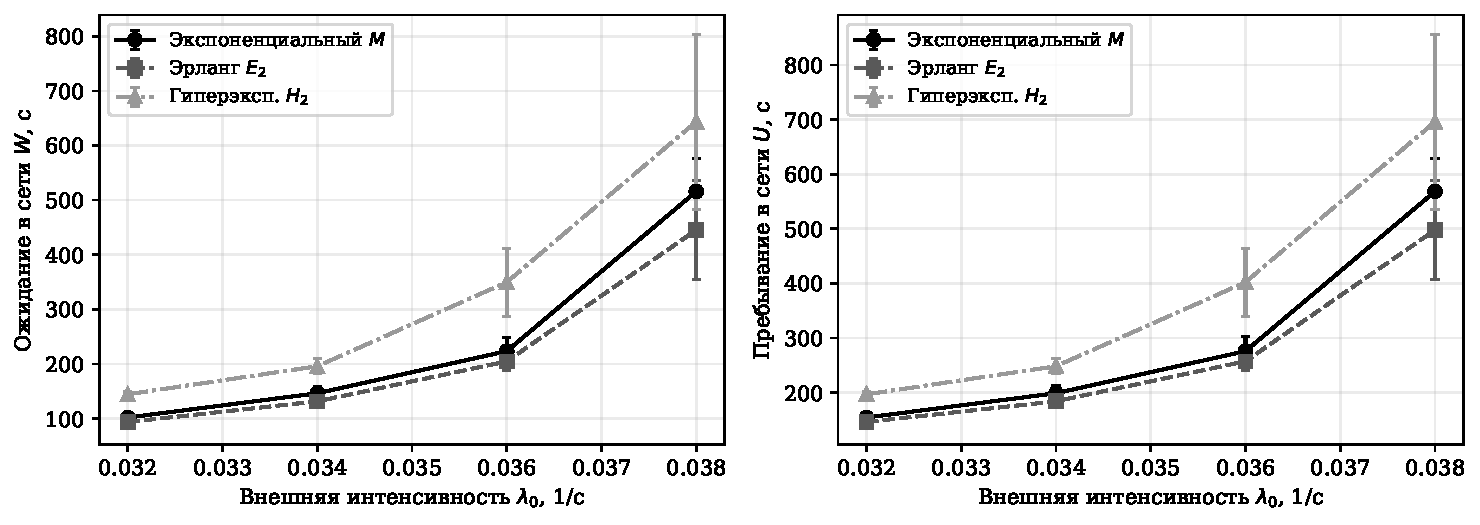
\includegraphics[width=\textwidth]{figures/open.pdf}\caption{Характеристики РСеМО при увеличении внешней интенсивности}\end{figure}


При экспоненциальном обслуживании узел У3 имеет характеристики M/M/1.
\begin{equation}
\rho_3=25\lambda_0,\qquad
u_3=\frac{b_3}{1-\rho_3},\qquad
w_3=u_3-b_3,\qquad
U=\sum_j\alpha_j u_j,\quad W=\sum_j\alpha_j w_j.
\end{equation}
Быстрый рост времени вблизи предельной интенсивности вызван множителем \(1/(1-\rho_3)\). Пропускная способность ограничена У3, хотя во внешнем потоке среднее число заявок в секунду остаётся небольшим.

\begin{center}\small\renewcommand{\arraystretch}{1.3}
\begin{tabular}{|l|c|c|c|c|}\hline
Закон У3 & Входной поток & \(\lambda_0\) & \(W\), с & \(U\), с\\\hline
\(M\) & П & 0,036717 & 270,50 & 322,81\\\hline
\(M\) & Детерм. & 0,036717 & 185,14 & 237,60\\\hline
\(E_2\) & П & 0,037235 & 315,07 & 367,64\\\hline
\(E_2\) & Детерм. & 0,037235 & 196,00 & 248,44\\\hline
\(H_2\) & П & 0,035539 & 302,37 & 354,85\\\hline
\(H_2\) & Детерм. & 0,035539 & 213,92 & 266,34\\\hline
\end{tabular}\end{center}

\concl{При сохранении средней интенсивности детерминированный вход уменьшает ожидание и пребывание. Он устраняет вариацию внешних поступлений, но случайные повторные посещения узлов сохраняются. При общем \(\lambda_0\) рост вариации обслуживания в У3 усиливает ожидание; это видно в серии по интенсивности, где средние входы у всех законов одинаковы.}

\section{Узловые характеристики, распределения и выводы}
Для каждой сети регистрируются загрузка узла, средняя длина очереди, число заявок, производительность, ожидание и пребывание. Ниже приведены сетевые и узловые оценки при \(M=3\); полные таблицы всех вариантов сохранены в CSV.

\noindent\begin{minipage}{\textwidth}\noindent\hfill Форма 2\par\begin{center}\textbf{Результаты имитационного моделирования для ЗСеМО}\end{center}
\noindent Экспоненциальная сеть \(M\) и неэкспоненциальная \(E_2\) в У3.\par 
Количество измеряемых завершённых циклов: 30000 в каждом из восьми повторений. 
Число заявок в сети \(M=3\). 
Средняя длительность измеряемого окна: \(T_M=817108,9\) с, \(T_{E_2}=805730,2\) с. Времена отдельных прогонов сохранены в \texttt{network\_protocols.csv}.\par
\begin{center}\small\renewcommand{\arraystretch}{1.3}
\resizebox{\textwidth}{!}{\begin{tabular}{|l|c|c|c|c|c|c|c|c|}\hline
\shortstack{Характе-\\ристики\\СеМО} & \shortstack{Экспон.\\У1} & \shortstack{Экспон.\\У2} & \shortstack{Экспон.\\У3} & \shortstack{Экспон.\\Сеть} & \shortstack{\(E_2\)\\У1} & \shortstack{\(E_2\)\\У2} & \shortstack{\(E_2\)\\У3} & \shortstack{\(E_2\)\\Сеть}\\\hline
Загрузка \(\rho\) & 0,1836 & 0,2062 & 0,9181 & -- & 0,1861 & 0,2092 & 0,9306 & --\\\hline
\shortstack{Длина\\очереди \(l\)} & 0,0309 & 0,0000 & 1,0429 & 1,0737 & 0,0226 & 0,0000 & 1,0240 & 1,0466\\\hline
\shortstack{Производи-\\тельность, с\(^{-1}\)} & 0,1836 & 0,0550 & 0,0918 & 0,0367 & 0,1862 & 0,0558 & 0,0931 & 0,0372\\\hline
\shortstack{Время\\ожидания, с} & 0,1679 & 0,0000 & 11,3549 & 29,2451 & 0,1215 & 0,0000 & 10,9954 & 28,1133\\\hline
\shortstack{Время\\пребывания, с} & 1,1674 & 14,9894 & 21,3498 & 81,7117 & 1,1210 & 14,9892 & 20,9874 & 80,5733\\\hline
\end{tabular}}\end{center}

\end{minipage}\par\medskip
\noindent\begin{minipage}{\textwidth}\noindent\hfill Форма 2\par\begin{center}\textbf{Результаты имитационного моделирования для ЗСеМО}\end{center}
\noindent Экспоненциальная сеть \(M\) и неэкспоненциальная \(H_2\) в У3.\par 
Количество измеряемых завершённых циклов: 30000 в каждом из восьми повторений. 
Число заявок в сети \(M=3\). 
Средняя длительность измеряемого окна: \(T_M=817108,9\) с, \(T_{H_2}=844234,4\) с. Времена отдельных прогонов сохранены в \texttt{network\_protocols.csv}.\par
\begin{center}\small\renewcommand{\arraystretch}{1.3}
\resizebox{\textwidth}{!}{\begin{tabular}{|l|c|c|c|c|c|c|c|c|}\hline
\shortstack{Характе-\\ристики\\СеМО} & \shortstack{Экспон.\\У1} & \shortstack{Экспон.\\У2} & \shortstack{Экспон.\\У3} & \shortstack{Экспон.\\Сеть} & \shortstack{\(H_2\)\\У1} & \shortstack{\(H_2\)\\У2} & \shortstack{\(H_2\)\\У3} & \shortstack{\(H_2\)\\Сеть}\\\hline
Загрузка \(\rho\) & 0,1836 & 0,2062 & 0,9181 & -- & 0,1777 & 0,1998 & 0,8914 & --\\\hline
\shortstack{Длина\\очереди \(l\)} & 0,0309 & 0,0000 & 1,0429 & 1,0737 & 0,0379 & 0,0000 & 1,0945 & 1,1324\\\hline
\shortstack{Производи-\\тельность, с\(^{-1}\)} & 0,1836 & 0,0550 & 0,0918 & 0,0367 & 0,1778 & 0,0533 & 0,0890 & 0,0355\\\hline
\shortstack{Время\\ожидания, с} & 0,1679 & 0,0000 & 11,3549 & 29,2451 & 0,2130 & 0,0000 & 12,3031 & 31,8630\\\hline
\shortstack{Время\\пребывания, с} & 1,1674 & 14,9894 & 21,3498 & 81,7117 & 1,2125 & 14,9842 & 22,3236 & 84,4205\\\hline
\end{tabular}}\end{center}

\end{minipage}\par\medskip
\noindent\begin{minipage}{\textwidth}\noindent\hfill Форма 3\par\begin{center}\textbf{Результаты имитационного моделирования для РСеМО}\end{center}
\noindent Экспоненциальная сеть \(M\) и неэкспоненциальная \(E_2\) в У3.\par 
Количество измеряемых завершённых циклов: 40000 в каждом из восьми повторений. 
Вход простейший, \(\lambda_{0,M}=0,036717\), \(\lambda_{0,E_2}=0,037235\) с\(^{-1}\). 
Средняя длительность измеряемого окна: \(T_M=1090901,1\) с, \(T_{E_2}=1074827,1\) с. Времена отдельных прогонов сохранены в \texttt{network\_protocols.csv}.\par
\begin{center}\small\renewcommand{\arraystretch}{1.3}
\resizebox{\textwidth}{!}{\begin{tabular}{|l|c|c|c|c|c|c|c|c|}\hline
\shortstack{Характе-\\ристики\\СеМО} & \shortstack{Экспон.\\У1} & \shortstack{Экспон.\\У2} & \shortstack{Экспон.\\У3} & \shortstack{Экспон.\\Сеть} & \shortstack{\(E_2\)\\У1} & \shortstack{\(E_2\)\\У2} & \shortstack{\(E_2\)\\У3} & \shortstack{\(E_2\)\\Сеть}\\\hline
Загрузка \(\rho\) & 0,1826 & 0,2050 & 0,9163 & -- & 0,1864 & 0,2095 & 0,9327 & --\\\hline
\shortstack{Длина\\очереди \(l\)} & 0,0406 & 0,0029 & 9,8911 & 9,9346 & 0,0330 & 0,0019 & 11,7101 & 11,7450\\\hline
\shortstack{Число заявок\\в системе \(m\)} & 0,2233 & 0,8227 & 10,8074 & 11,8534 & 0,2194 & 0,8400 & 12,6429 & 13,7022\\\hline
\shortstack{Время\\ожидания, с} & 0,2225 & 0,0483 & 108,0181 & 270,5030 & 0,1767 & 0,0349 & 125,3257 & 315,0714\\\hline
\shortstack{Время\\пребывания, с} & 1,2217 & 15,0219 & 118,0321 & 322,8145 & 1,1759 & 15,0013 & 135,3319 & 367,6445\\\hline
\end{tabular}}\end{center}

\end{minipage}\par\medskip
\noindent\begin{minipage}{\textwidth}\noindent\hfill Форма 3\par\begin{center}\textbf{Результаты имитационного моделирования для РСеМО}\end{center}
\noindent Экспоненциальная сеть \(M\) и неэкспоненциальная \(H_2\) в У3.\par 
Количество измеряемых завершённых циклов: 40000 в каждом из восьми повторений. 
Вход простейший, \(\lambda_{0,M}=0,036717\), \(\lambda_{0,H_2}=0,035539\) с\(^{-1}\). 
Средняя длительность измеряемого окна: \(T_M=1090901,1\) с, \(T_{H_2}=1123416,8\) с. Времена отдельных прогонов сохранены в \texttt{network\_protocols.csv}.\par
\begin{center}\small\renewcommand{\arraystretch}{1.3}
\resizebox{\textwidth}{!}{\begin{tabular}{|l|c|c|c|c|c|c|c|c|}\hline
\shortstack{Характе-\\ристики\\СеМО} & \shortstack{Экспон.\\У1} & \shortstack{Экспон.\\У2} & \shortstack{Экспон.\\У3} & \shortstack{Экспон.\\Сеть} & \shortstack{\(H_2\)\\У1} & \shortstack{\(H_2\)\\У2} & \shortstack{\(H_2\)\\У3} & \shortstack{\(H_2\)\\Сеть}\\\hline
Загрузка \(\rho\) & 0,1826 & 0,2050 & 0,9163 & -- & 0,1777 & 0,1996 & 0,8924 & --\\\hline
\shortstack{Длина\\очереди \(l\)} & 0,0406 & 0,0029 & 9,8911 & 9,9346 & 0,0501 & 0,0052 & 10,7026 & 10,7580\\\hline
\shortstack{Число заявок\\в системе \(m\)} & 0,2233 & 0,8227 & 10,8074 & 11,8534 & 0,2279 & 0,8038 & 11,5950 & 12,6266\\\hline
\shortstack{Время\\ожидания, с} & 0,2225 & 0,0483 & 108,0181 & 270,5030 & 0,2821 & 0,0989 & 120,2108 & 302,3671\\\hline
\shortstack{Время\\пребывания, с} & 1,2217 & 15,0219 & 118,0321 & 322,8145 & 1,2810 & 15,0650 & 130,2321 & 354,8513\\\hline
\end{tabular}}\end{center}

\end{minipage}\par\medskip
\begin{figure}[H]\centering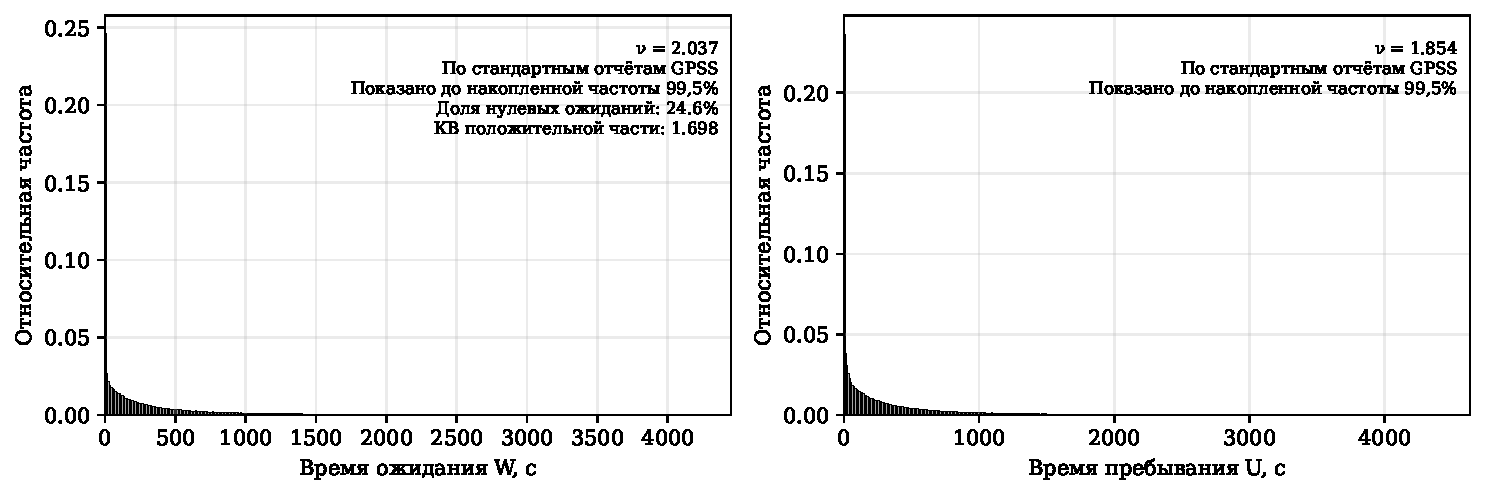
\includegraphics[width=\textwidth]{figures/hist_network.pdf}\caption{Распределения времени в открытой сети с \(H_2\) в У3 при загрузке узкого места 0,9}\end{figure}

В сетевом опыте доля нулевых ожиданий равна 0,246, КВ положительной части -- 1,698. Для этой положительной части допустима гипотеза двухмоментной аппроксимации \(H_2\); точный закон по гистограмме не устанавливается.

Коэффициенты вариации и гистограммы времени ожидания и пребывания в РСеМО показывают правую асимметрию. \(H_2\) может использоваться как двухмоментная аппроксимация положительной части при \(\nu>1\). В замкнутой сети изменение закона У3 влияет и на пропускную способность, поскольку меняется вероятность его простоя при конечном \(M\). В устойчивой открытой сети долговременная производительность равна внешней интенсивности; закон обслуживания главным образом меняет очереди и времена.

\begin{enumerate}
\item Имитационная GPSS-модель выбранной СМО воспроизводит шесть стационарных характеристик УИР 2; численные расхождения в процентах приведены в контрольной таблице.
\item Для исходной трассы и её аппроксимации потери и ожидание выше, чем для простейшего потока с тем же средним интервалом. Причина -- высокая вариация интервалов и серии близких поступлений.
\item Увеличение накопителя снижает отказы ценой большего ожидания. Отсутствие отказов в конечном опыте не означает их нулевую теоретическую вероятность.
\item В сети М1 узкое место -- У3. Предел производительности равен 0,04 цикла/с. По критерию приращения менее 1\% получено \(M^*=6\).
\item Ускорение или распараллеливание У3 увеличивает пропускную способность. При насыщении дальнейшее увеличение числа заявок удлиняет очереди, почти не увеличивая производительность.
\item При равном внешнем потоке открытая сеть имеет большее ожидание, поскольку число заявок в ней не ограничено. При приближении к предельной интенсивности ожидание резко возрастает.
\end{enumerate}

\newpage\appendix
\section{Текст GPSS-модели исходной СМО}
Ниже приведён текст модели для контрольного сравнения с УИР 2. Единица модельного времени -- секунда. Варианты трассы, аппроксимации, обслуживания и буферов находятся в папке \texttt{gpss}. Тексты включают команды разгона, сброса статистики и измерения. Команда \texttt{EXIT 1} рассчитана на пакетный запуск; для интерактивной демонстрации её следует убрать, чтобы окно результатов оставалось открытым.
\begin{multicols}{2}\lstinputlisting{../gpss/smo_baseline.txt}\end{multicols}

\newpage\section{Текст GPSS-модели замкнутой сети: \(M\) в У3}
Во всех вариантах У1 и У2 обслуживают экспоненциально. 
В сети \(M=3\) заявки. Возврат через условный узел «0» завершает цикл. Копия транзакта уменьшает счётчик завершений, исходный транзакт продолжает циркуляцию. 
Для \(E_2\) суммируются две экспоненциальные фазы; для \(H_2\) выбирается одна из двух ветвей с КВ = 2. Модель прошла трансляцию и выполнение в GPSS. Полные команды независимых повторений находятся в \texttt{gpss-native/series}.\par
\begin{multicols}{2}\lstinputlisting{../gpss/closed_M_M3.txt}\end{multicols}
\newpage\section{Текст GPSS-модели замкнутой сети: \(E_2\) в У3}
Во всех вариантах У1 и У2 обслуживают экспоненциально. 
В сети \(M=3\) заявки. Возврат через условный узел «0» завершает цикл. Копия транзакта уменьшает счётчик завершений, исходный транзакт продолжает циркуляцию. 
Для \(E_2\) суммируются две экспоненциальные фазы; для \(H_2\) выбирается одна из двух ветвей с КВ = 2. Модель прошла трансляцию и выполнение в GPSS. Полные команды независимых повторений находятся в \texttt{gpss-native/series}.\par
\begin{multicols}{2}\lstinputlisting{../gpss/closed_E2_M3.txt}\end{multicols}
\newpage\section{Текст GPSS-модели замкнутой сети: \(H_2\) в У3}
Во всех вариантах У1 и У2 обслуживают экспоненциально. 
В сети \(M=3\) заявки. Возврат через условный узел «0» завершает цикл. Копия транзакта уменьшает счётчик завершений, исходный транзакт продолжает циркуляцию. 
Для \(E_2\) суммируются две экспоненциальные фазы; для \(H_2\) выбирается одна из двух ветвей с КВ = 2. Модель прошла трансляцию и выполнение в GPSS. Полные команды независимых повторений находятся в \texttt{gpss-native/series}.\par
\begin{multicols}{2}\lstinputlisting{../gpss/closed_H2_M3.txt}\end{multicols}
\newpage\section{Текст GPSS-модели разомкнутой сети: \(M\) в У3}
Во всех вариантах У1 и У2 обслуживают экспоненциально. 
Интенсивность простейшего внешнего потока равна производительности соответствующей замкнутой сети при \(M=3\). 
Для \(E_2\) суммируются две экспоненциальные фазы; для \(H_2\) выбирается одна из двух ветвей с КВ = 2. Модель прошла трансляцию и выполнение в GPSS. Полные команды независимых повторений находятся в \texttt{gpss-native/series}.\par
\begin{multicols}{2}\lstinputlisting{../gpss/open_matched_M_M.txt}\end{multicols}
\newpage\section{Текст GPSS-модели разомкнутой сети: \(E_2\) в У3}
Во всех вариантах У1 и У2 обслуживают экспоненциально. 
Интенсивность простейшего внешнего потока равна производительности соответствующей замкнутой сети при \(M=3\). 
Для \(E_2\) суммируются две экспоненциальные фазы; для \(H_2\) выбирается одна из двух ветвей с КВ = 2. Модель прошла трансляцию и выполнение в GPSS. Полные команды независимых повторений находятся в \texttt{gpss-native/series}.\par
\begin{multicols}{2}\lstinputlisting{../gpss/open_matched_E2_M.txt}\end{multicols}
\newpage\section{Текст GPSS-модели разомкнутой сети: \(H_2\) в У3}
Во всех вариантах У1 и У2 обслуживают экспоненциально. 
Интенсивность простейшего внешнего потока равна производительности соответствующей замкнутой сети при \(M=3\). 
Для \(E_2\) суммируются две экспоненциальные фазы; для \(H_2\) выбирается одна из двух ветвей с КВ = 2. Модель прошла трансляцию и выполнение в GPSS. Полные команды независимых повторений находятся в \texttt{gpss-native/series}.\par
\begin{multicols}{2}\lstinputlisting{../gpss/open_matched_H2_M.txt}\end{multicols}
\end{document}